\documentclass[%
<<<<<<< Updated upstream
11pt,%
%oneside,%
twoside,%
%twocolumn,%
titlepage,%
%fleqn,%
%a4page,%
german,%
headsepline%
]{scrartcl}

%\usepackage{fancyhdr}
%\usepackage{scrpage}
\usepackage{lastpage}
\usepackage{geometry}
\usepackage{graphicx}
\usepackage[utf8]{inputenc}
\usepackage[ngerman]{babel}
\usepackage{lscape}
\usepackage[framemethod=TikZ]{mdframed}
\usepackage[most]{tcolorbox}
\usepackage{mymath}
\usepackage{units}
\usepackage{nicefrac}
\usepackage{pgf,tikz,pgfplots}
\pgfplotsset{compat=1.14}
\usepackage{mathrsfs}
\usetikzlibrary{arrows}
=======
%draft,
11pt,%
twoside,%
titlepage,%
swissgerman,%
headsepline%
]{scrartcl}

\usepackage{lastpage}
\usepackage{amsthm}
\usepackage{amssymb}
\usepackage{geometry}
\usepackage{graphicx}
\usepackage[dvipsnames]{xcolor}
\usepackage[utf8]{inputenc}
\usepackage[swissgerman]{babel}
\usepackage{lscape}
\usepackage[framemethod=TikZ]{mdframed}
\usepackage[most]{tcolorbox}
\usepackage{enumerate}
\usepackage{units}
\usepackage{nicefrac}
\usepackage{pgf,tikz}
\usepackage{tikz-3dplot}
\usepackage{tkz-euclide}
\usetikzlibrary{arrows}
\usetikzlibrary{arrows.meta}
\usetikzlibrary{patterns}
\usetikzlibrary{positioning}
\usetikzlibrary{shadows}
\usetikzlibrary{quotes, angles}
>>>>>>> Stashed changes
\usepackage{colortbl}
\usepackage{hhline}
\usepackage{multirow}
\usepackage[extendedchars]{grffile}
\usepackage{caption}
\usepackage{multicol,calc}
\usepackage{blindtext}
\usepackage{pdfpages}
\usepackage{hyperref}
<<<<<<< Updated upstream
\usepackage{tikz-er2}
\usepackage{framed}
\usetikzlibrary{arrows}
\usetikzlibrary{positioning}
\usetikzlibrary{shadows}

\usepackage{marginnote}
\usepackage[]{qrcode}
\qrset{height=9ex}

%\usepackage{romannum}
\usepackage{longtable}
\usepackage{listings}
\usepackage{wrapfig}
\usepackage{svg}
=======
\usepackage{framed}

\usepackage{marginnote}
\usepackage{qrcode}
\qrset{height=9ex}

\usepackage{longtable}
\usepackage{listings}
\usepackage{wrapfig}

\usepackage{fontawesome} % Oder FontAwesome, falls du ein Augensymbol aus einer
\newcommand{\faEyeLightGray}{\textcolor{lightgray}{\faEye}} % Custom command for the gray eye icon
\newcommand{\faReturnGray}{\textcolor{gray}{\faMailReply}} % Custom command for the gray eye icon
\usepackage{pifont} % weitere Zeichen

% package für plots mit dem Befehl axes
\usepackage{pgfplots}

>>>>>>> Stashed changes


% Command, um Tabellen-Spalten anzupassen
\newcommand{\spaltenheight}{\rule{0mm}{3ex}}
\newcommand{\spaltenwidth}{\rule{3cm}{0mm}}
\newcommand{\spaltensep}{\\[1ex]}
%\arrayrulecolor{darkgreen}
\doublerulesepcolor{white}

% colors
\definecolor{lightyellow}{rgb}{1,1,0.8}
\definecolor{Gray}{gray}{0.9}
<<<<<<< Updated upstream
\definecolor{darkblue}{rgb}{0,0,0.55}
\definecolor{firebrick}{rgb}{0.7,0.13,0.13}
\definecolor{seagreen}{rgb}{0.18,0.55,0.34}
\pagestyle{headings} % gemachte Einstellungen anwenden

% Farbig umrahmte Umgebung Satz
 
 \definecolor{myblizzardblue}{HTML}{87CEEB}

\newcounter{satzz}[section]\setcounter{satzz}{0}
\renewcommand{\thesatz}{\arabic{section}.\arabic{satzz}}

\newenvironment{csatz}[2][]{%
=======
\definecolor{lightgray}{rgb}{0.7, 0.7, 0.7}
\definecolor{darkblue}{rgb}{0,0,0.55}
\definecolor{firebrick}{rgb}{0.7,0.13,0.13}
\definecolor{seagreen}{rgb}{0.18,0.55,0.34}
\definecolor{emerald}{HTML}{50C878} % color of Definition
\definecolor{whitesmoke}{HTML}{F5F5F5} % background for environments
\definecolor{myblizzardblue}{HTML}{87CEEB} % color of Satz

% Für Definitionen im Fliesstext
\newcommand{\definition}[1]{\colorbox{emerald}{#1}}
% Für Regeln im Fliesstext
\newcommand{\regel}[1]{\colorbox{myblizzardblue}{#1}}
% Für Merke/Achtungs im Fliesstext
\newcommand{\merke}[1]{\colorbox{firebrick}{#1}}
% Geogebra-Link
\newcommand{\geogebralink}{\href{https://www.geogebra.org/calculator}{\texttt{geogebra.org}}}

% Umgebungen
\theoremstyle{definition}
    \newtheorem{bsp}{Beispiel}[subsection] % Beispiele
    \newtheorem{bem}{Bemerkung}[subsection] % Bemerkungen
\theoremstyle{plain}
    \newtheorem{thm}{Theorem} % Theorem [subsection]
    \newtheorem{satz}{Satz} % Satz [subsection]

% Umgebung lsg mit dynamischer Referenzierung und Label
\newcommand{\concatueb}[1]{ueb:#1}% Definition für concatueb
\newcommand{\concatlsg}[1]{lsg:#1}% Definition für concatlsg

\newcounter{uebcounter}[section]
\renewcommand{\theuebcounter}{\thesection.\arabic{uebcounter}}  % Zählerformat: Abschnitt.Übung

\newenvironment{lsg}[1]{%
    \par\noindent\textbf{Notizen zu Übung \theuebcounter\label{\concatlsg{#1}}}
    \hfill\hyperref[\concatueb{#1}]{\faReturnGray}\par % Hyperref-Button zurück zur Übung
}{%
    \par%
}

\newenvironment{uebenv}[1]{%
    \refstepcounter{uebcounter}
    \par\noindent\textbf{Übung \theuebcounter.}%
    \label{\concatueb{#1}}\hfill\hyperref[\concatlsg{#1}]{\faEyeLightGray}\par
}{%
    \par
}

% Umgebung für Definitionen
\newcounter{deff}[section]\setcounter{deff}{0}
\renewcommand{\thedeff}{\arabic{section}.\arabic{deff}}

\newenvironment{cdef}[1][]{%
    \refstepcounter{deff} 
    \ifstrempty{#1}%
    % if condition (without title)
    {\mdfsetup{%
        frametitle={%
            \tikz[baseline=(current bounding box.east),outer sep=0pt]
            \node[anchor=east,rectangle,fill=emerald]
            {\strut Definition~\thedeff};}
        }%
    % else condition (with title)
    }{\mdfsetup{%
        frametitle={%
            \tikz[baseline=(current bounding box.east),outer sep=0pt]
            \node[anchor=east,rectangle,fill=emerald]
            {\strut Definition~\thedeff:~#1};}%
        }%
    }%
% for both conditions
    \mdfsetup{%
        innertopmargin=10pt,linecolor=emerald,%
        backgroundcolor=whitesmoke,%
        linewidth=2pt,topline=true,%
        frametitleaboveskip=\dimexpr-\ht\strutbox\relax%
    } 
\begin{mdframed}[]\relax}{%
\end{mdframed}}

% Farbig umrahmte Umgebung Satz
\newcounter{satzz}[section]\setcounter{satzz}{0}
\renewcommand{\thesatz}{\arabic{section}.\arabic{satzz}}

\newenvironment{csatz}[1][]{%
>>>>>>> Stashed changes
    \refstepcounter{satzz}
 
    \ifstrempty{#1}%
    % if condition (without title)
    {\mdfsetup{%
        frametitle={%
            \tikz[baseline=(current bounding box.east),outer sep=0pt]
            \node[anchor=east,rectangle,fill=myblizzardblue]
            {\strut Satz~\thesatz};}
        }%
    % else condition (with title)
    }{\mdfsetup{%
        frametitle={%
            \tikz[baseline=(current bounding box.east),outer sep=0pt]
            \node[anchor=east,rectangle,fill=myblizzardblue]
            {\strut Satz~\thesatz:~#1};}%
        }%
    }%
% for both conditions
    \mdfsetup{%
        innertopmargin=10pt,linecolor=myblizzardblue,%
        backgroundcolor=whitesmoke,%
        linewidth=2pt,topline=true,%
        frametitleaboveskip=\dimexpr-\ht\strutbox\relax%
    }
<<<<<<< Updated upstream
 
\begin{mdframed}[]\relax}{%
\end{mdframed}}

% Farbig umrahmte Umgebung Theorem
 
\definecolor{mygraphblue}{HTML}{84B7E1}
\definecolor{whitesmoke}{HTML}{F5F5F5}

\newcounter{theo}[section]\setcounter{theo}{0}
\renewcommand{\thetheo}{\arabic{section}.\arabic{theo}}

\newenvironment{ctheo}[2][]{%
    \refstepcounter{theo}
 
    \ifstrempty{#1}%
    % if condition (without title)
    {\mdfsetup{%
        frametitle={%
            \tikz[baseline=(current bounding box.east),outer sep=0pt]
            \node[anchor=east,rectangle,fill=mygraphblue]
            {\strut Theorem~\thetheo};}
        }%
    % else condition (with title)
    }{\mdfsetup{%
        frametitle={%
            \tikz[baseline=(current bounding box.east),outer sep=0pt]
            \node[anchor=east,rectangle,fill=mygraphblue]
            {\strut Theorem~\thetheo:~#1};}%
        }%
    }%
% for both conditions
    \mdfsetup{%
        innertopmargin=10pt,linecolor=mygraphblue,%
        backgroundcolor=whitesmoke,%
        linewidth=2pt,topline=true,%
        frametitleaboveskip=\dimexpr-\ht\strutbox\relax%
    }
 
\begin{mdframed}[]\relax}{%
\end{mdframed}}

% Farbig umrahmte Umgebung Definition
 
 \definecolor{emerald}{HTML}{50C878}

\newcounter{deff}[section]\setcounter{deff}{0}
\renewcommand{\thedeff}{\arabic{section}.\arabic{deff}}

\newenvironment{cdef}[2][]{%
    \refstepcounter{deff}
 
    \ifstrempty{#1}%
    % if condition (without title)
    {\mdfsetup{%
        frametitle={%
            \tikz[baseline=(current bounding box.east),outer sep=0pt]
            \node[anchor=east,rectangle,fill=emerald]
            {\strut Definition~\thedeff};}
        }%
    % else condition (with title)
    }{\mdfsetup{%
        frametitle={%
            \tikz[baseline=(current bounding box.east),outer sep=0pt]
            \node[anchor=east,rectangle,fill=emerald]
            {\strut Definition~\thedeff:~#1};}%
        }%
    }%
% for both conditions
    \mdfsetup{%
        innertopmargin=10pt,linecolor=emerald,%
        backgroundcolor=whitesmoke,%
        linewidth=2pt,topline=true,%
        frametitleaboveskip=\dimexpr-\ht\strutbox\relax%
    }
 
\begin{mdframed}[]\relax}{%
\end{mdframed}}

% Farbig umrahmte Umgebung Achtung
 
 \definecolor{mygraphred}{HTML}{E26A6A}

\newcounter{merkee}[section]\setcounter{merkee}{0}
\renewcommand{\themerkee}{\arabic{section}.\arabic{merkee}}

\newenvironment{cachtung}[2][]{%
    \refstepcounter{merkee}
 
    \ifstrempty{#1}%
    % if condition (without title)
    {\mdfsetup{%
        frametitle={%
            \tikz[baseline=(current bounding box.east),outer sep=0pt]
            \node[anchor=east,rectangle,fill=mygraphred]
            {\strut Achtung};}
        }%
    % else condition (with title)
    }{\mdfsetup{%
        frametitle={%
            \tikz[baseline=(current bounding box.east),outer sep=0pt]
            \node[anchor=east,rectangle,fill=mygraphred]
            {\strut Achtung:~#1};}%
        }%
    }%
% for both conditions
    \mdfsetup{%
        innertopmargin=10pt,linecolor=mygraphred,%
        backgroundcolor=whitesmoke,%
        linewidth=2pt,topline=true,%
        frametitleaboveskip=\dimexpr-\ht\strutbox\relax%
    }
 
\begin{mdframed}[]\relax}{%
\end{mdframed}}

% Python Code
\usepackage{listings}
\lstset{language=Python,
        basicstyle=\ttfamily,
        keywordstyle=\color{blue},
        stringstyle=\color{red},
        commentstyle=\color{green},
        morecomment=[l][\color{magenta}]{\#}
}

\usepackage{fontawesome} % FontAwesome, falls du ein Augensymbol brauchst
\definecolor{lightgray}{rgb}{0.7, 0.7, 0.7}
\newcommand{\faEyeLightGray}{\textcolor{lightgray}{\faEye}} % Custom command for the gray eye icon

\subject{\includegraphics[width=0.618\textwidth]{pictures/apfelmaennchen.jpg}}
\title{Iterationen}
\subtitle{vom Repetitiven ins Chaos}
\author{}
\date{}
%\newtheorem{uebthm}{Übung}[section]
% Umgebung lsg mit dynamischer Referenzierung und Label
\newcommand{\concatueb}[1]{ueb:#1}% Definition für concatueb
\newcommand{\concatlsg}[1]{lsg:#1}% Definition für concatlsg

\newcounter{uebcounter}[section]
\renewcommand{\theuebcounter}{\thesection.\arabic{uebcounter}}  % Zählerformat: Abschnitt.Übung

% Definition einer Übungsumgebung mit dynamischen Labels
\newcommand{\uebh}[2]{%
 \refstepcounter{uebcounter} % Zählt den Übungscounter hoch
 \par\noindent\textbf{Übung \theuebcounter:}\label{\concatueb{#1}} % Label im Format "ueb:1"
    #2
    \hfill\hyperref[\concatlsg{#1}]{\faEyeLightGray}
    \vspace{\parskip}
}

\newenvironment{lsg}[1]{%
    \par\noindent\textbf{Notizen zu Übung \ref{\concatueb{#1}}.}%
    \label{\concatlsg{#1}}
}{%
    \par%
}

\newenvironment{uebenv}[1]{%
    \refstepcounter{uebcounter}
    \par\noindent\textbf{Übung \theuebcounter.}%
    \label{\concatueb{#1}}\hfill\hyperref[\concatlsg{#1}]{\faEyeLightGray}\par
}{%
    \par
}

\newcommand{\definition}[1]{\colorbox{emerald}{#1}}

\setlength{\parindent}{0pt}
=======
\begin{mdframed}[]\relax}{%
\end{mdframed}}

% kein Einzug bei neuem Abschnitt
\setlength{\parindent}{0pt} \setlength{\parskip}{1em}
\pagestyle{headings} % gemachte Einstellungen anwenden
>>>>>>> Stashed changes

\subject{\includegraphics[width=0.618\textwidth]{pictures/apfelmaennchen.jpg}}
\title{Iterationen}
\subtitle{vom Repetitiven ins Chaos}
\author{}
\date{}
\lowertitleback{
\includegraphics[height=1cm]{pictures/gymfmslerbermattlogo.eps}
\hfill%\copyright%
{\begin{tikzpicture}
  % Draw the rounded rectangle and clip the image to it
  \clip [rounded corners=5mm] (0,0) rectangle (1,1); % Adjust dimensions as needed
  \node at (0.5,0.5) {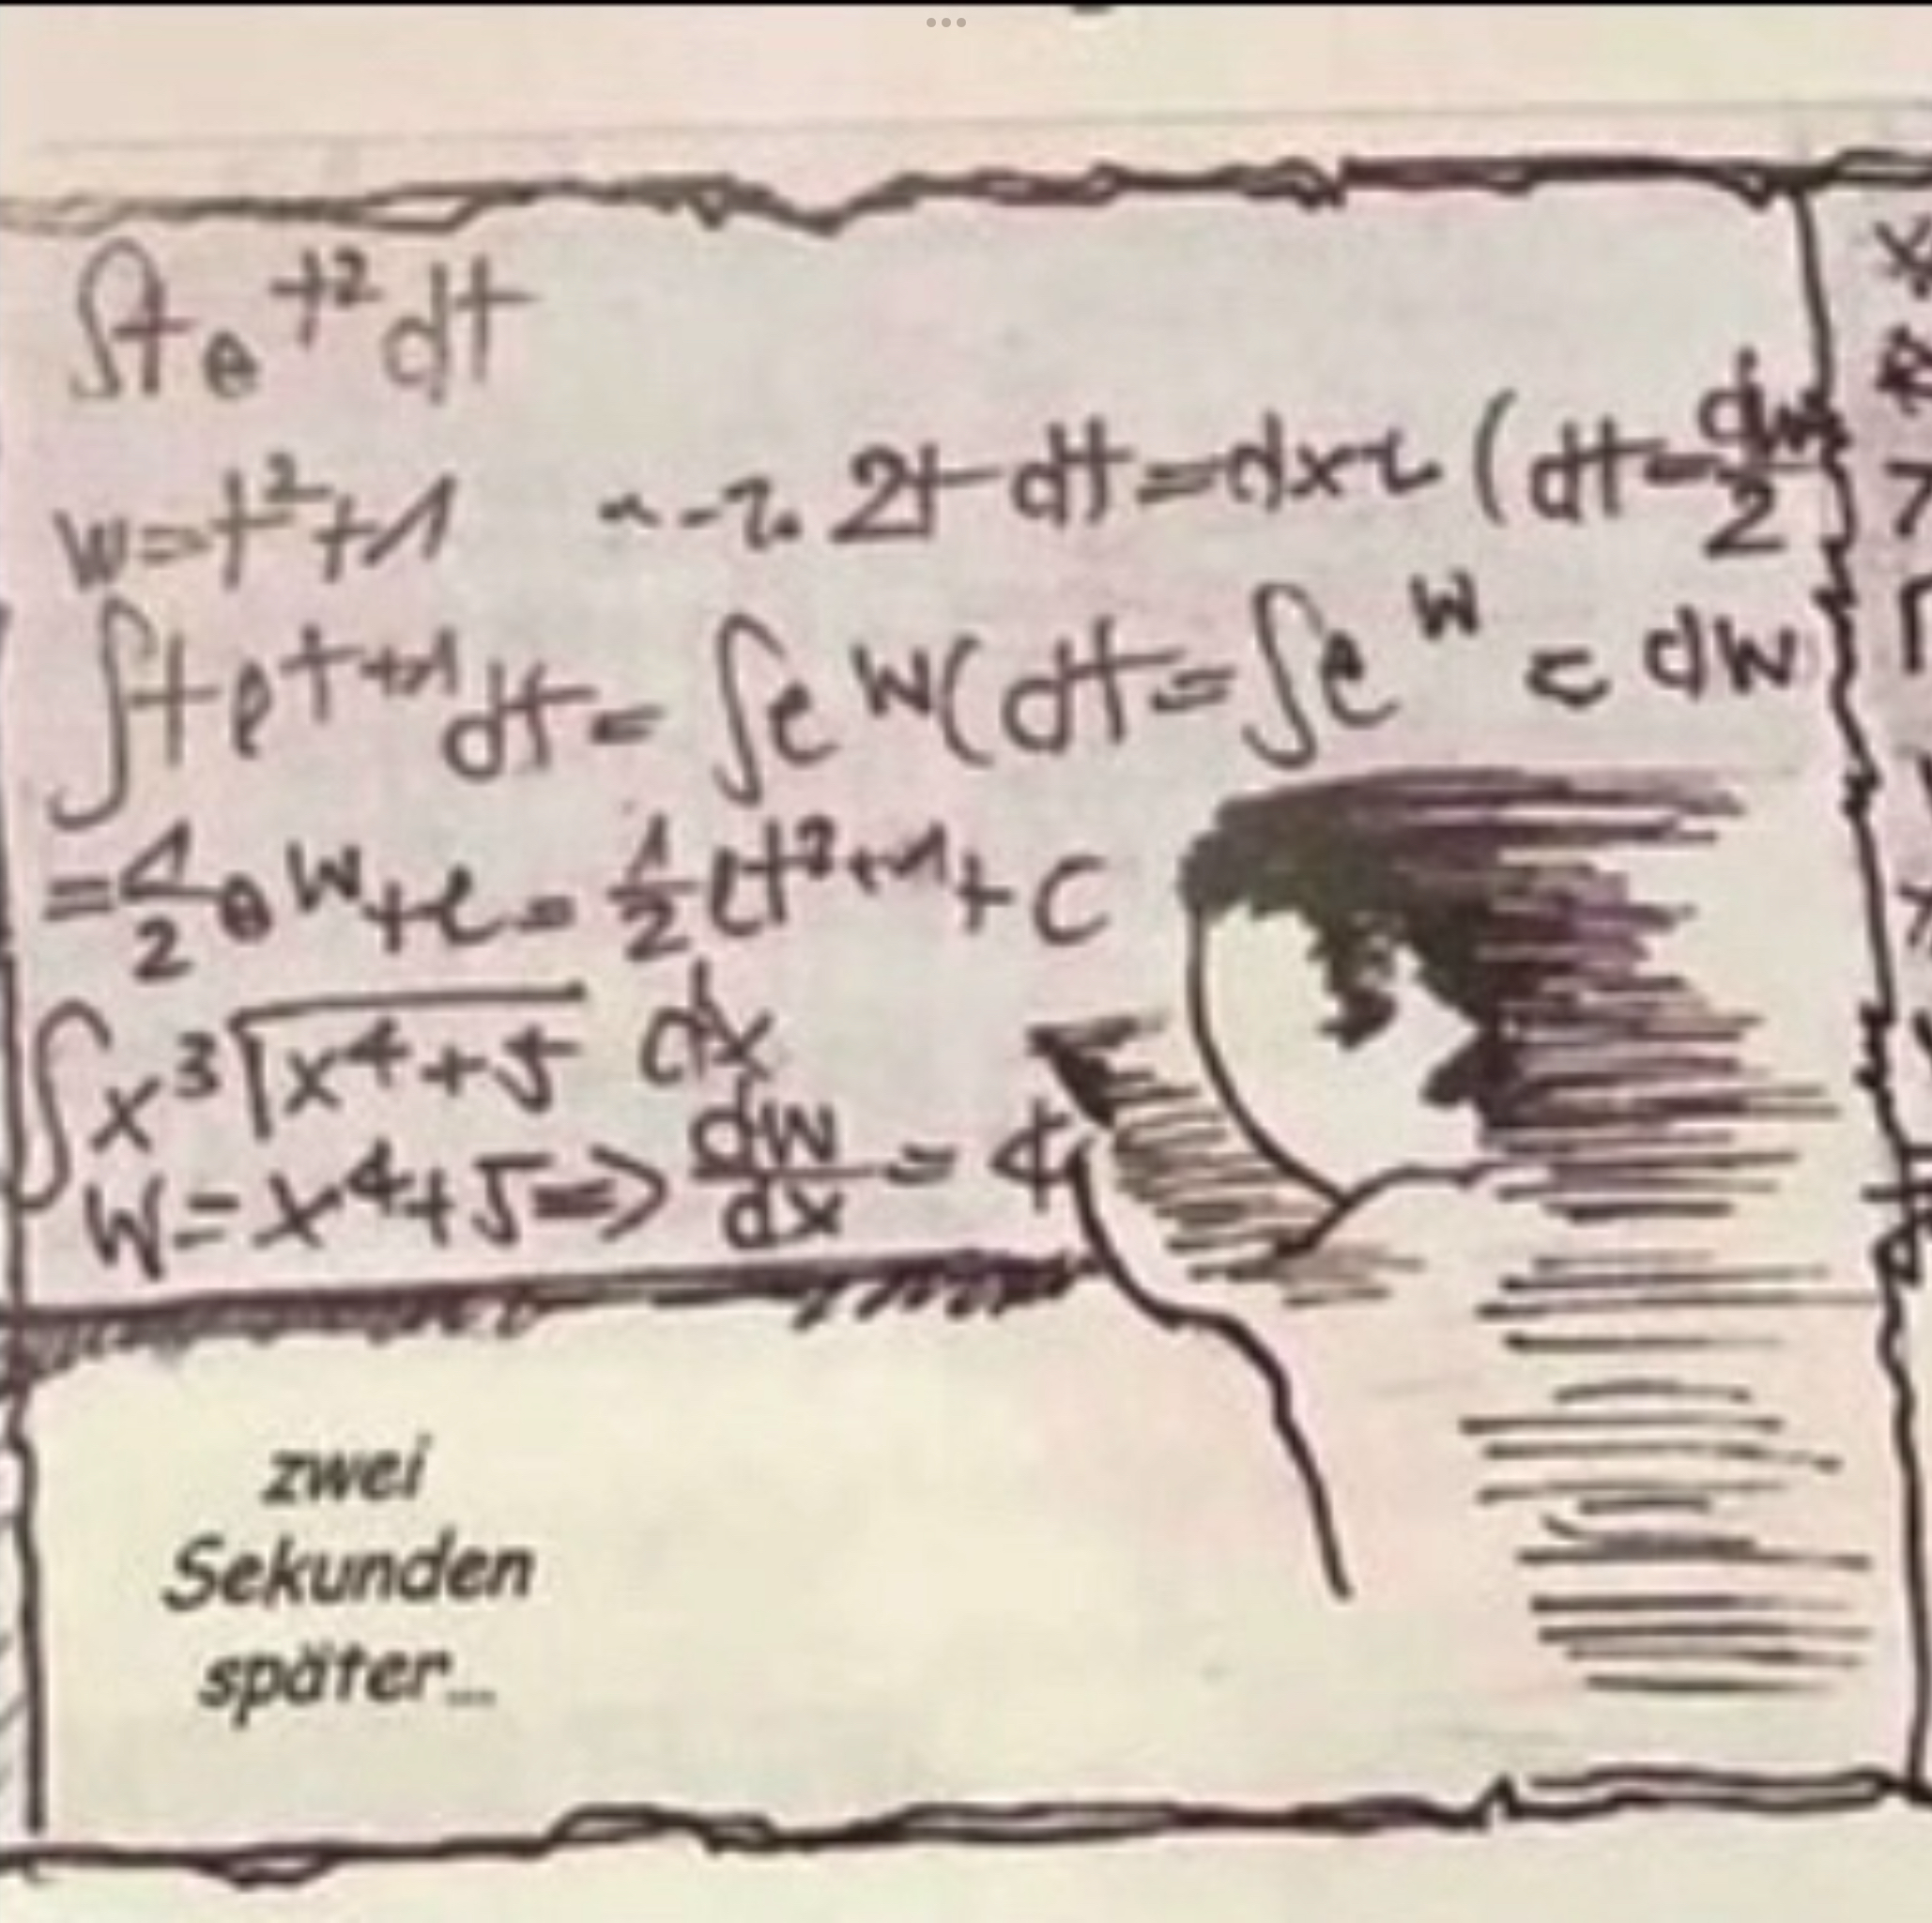
\includegraphics[width=1cm]{pictures/teacher_me_caricatur.png}}; % Adjust width and center image
\end{tikzpicture}}
}

\begin{document}
\maketitle
\tableofcontents
%\thispagestyle{empty}
\cleardoublepage
%\setcounter{page}{1}

\section{Erste Beispiele}

\subsection{Sierpinski Dreieck}

Wir spielen folgendes Spiel (Barnsley's Chaos Game):
\begin{quote}
Gegeben sei ein Dreieck mit den Eckpunkten $1,2,3$. Wir w\"ahlen einen beliebigen Startpunkt $x_0$, sowie einen beliebigen Punkt $P$, und berechnen mit der Vorschrift
$$x_1=\frac{x_0+P}{2}$$
den Punkt $x_1$. Fahren Sie nach diesem Schema fort, um weitere Punkte zu bestimmen.
\end{quote}
Am einfachsten geht's, wenn man sich rasch ein Programm schreibt, das obiges Verfahren ausführt.

\begin{lstlisting}
import random
import matplotlib.pyplot as plt

def sierpinski(n):
  vertices = [(0.0,0.0), (0.5,0.85), (1.0,0.0)]
  points = []
  x,y = random.choice(vertices) #Startpunkt
  
  for i in range(n):
    vx,vy = random.choice(vertices) #waehle zufaellige Ecke
    
    x = (vx+x)/2.0 #Mittelung
    y = (vy+y)/2.0
    
    points.append((x,y))
    
    plot(points)
\end{lstlisting}

\begin{figure}[h!]
  \centering
\includegraphics[width=0.382\textwidth]{pictures/sierpinski}
\caption{Sierpinski Dreieck, Struktur im Zufall}
\end{figure}

Noch ein Hinweis zur verblüffenden Tatsache, dass das Random Game gegen den Attraktor Sierpinski-Dreieck konvergiert. Klar und mit einfachen Argumenten wird dies im \href{https://www.youtube.com/watch?v=5nuYD2M2AX8}{YouTube Video von Robin Truax} erklärt.

Es gibt eine weitere, erstaunliche Beziehung zum Pascal'schen Dreieck, die ich von Agnes Scott habe. Und zwar kriegt man das Sierpinski-Dreieck-Muster, wenn man im Pascal'schen Dreieck alle geraden Zahlen mit einer Farbe markiert.

Dies sieht man wie folgt ein:
Bezeichne $P_n$ die ersten $2^n$ Zeilen des Pascal-Dreiecks (PD). Wir zeigen, dass $P_{n+1}$ aus 3 Kopien von $P_n$ besteht, die ein Dreieck mit geraden Koeffizienten umgeben. Die ersten $2^n$ Zeilen von $P_{n+1}$ sind natürlich identisch mit den ersten $2^n$ Zeilen von $P_n$. Wir wollen beweisen, dass für jeden Koeffizienten in $P_n$ die Koeffizienten an den entsprechenden Positionen in den unteren linken und unteren rechten Dreiecken von $P_{n+1}$ denselben Wert (mod 2) haben wie der Koeffizient in $P_n$.

Die Beweisgrundlage bildet das Theorem von Lucas. Das folgende klassische Theorem wurde 1890 von Édouard Lucas bewiesen:

\begin{csatz}[Lucas' Theorem]
Sei $p$ priom und $r,c$ in $p$-adischer Notation:
$$r=r_k\dots r_1r_0=r_0+r_1p+\dots+r_kp^k\quad(0\leq r_i<p)$$
$$c=c_k\dots c_1c_0=c_0+c_1p+\dots+c_kp^k\quad(0\leq c_i<p)$$
Dann gilt:
$$\binom{r}{c}=\binom{r_0}{c_0}\binom{r_1}{c_1}\dots\binom{r_k}{c_k}\mod(p)$$
\end{csatz}
Ferner gilt wie üblich $\binom{r}{c}=0$, falls $c>r$.

Um das Pascalsche Dreieck modulo 2 zu untersuchen, setzen wir $p=2$. Der Binomialkoeffizient 
$\binom{r}{c}$ in Zeile $r$ und Spalte $c$ von $P_n$ kann in binärer Darstellung geschrieben werden, da $r,c<2^n$:
$$r=r_{n-1}\dots r_1r_0,\quad c=c_{n-1}\dots c_1c_0\quad(r_i,c_i\in\{0,1\}.$$
In $P_n$ entspricht der Koeffizient an der unteren linken Ecke $\binom{2^n+r}{2^n+c}$ und an der unteren rechten Ecke $\binom{2^n+r}{c}$. Nach Lucas’ Theorem gilt:
$$\binom{2^n+r}{c}\equiv\binom{r}{c}\mod(2),\quad\binom{2^n+r}{2^n+c}\equiv\binom{r}{c}\mod(2).$$
Alle drei Binomialkoeffizienten haben somit denselben Wert modulo 2 und damit dieselbe Farbe im Pascalschen Dreieck (mod 2). Dies beweist den ersten Teil des rekursiven Verhaltens.

Wir zeigen nun, dass die drei äquivalenten Eckdreiecke von $P_{n+1}$ ein Dreieck aus geraden Zahlen umgeben. Die letzte Zeile von $P_n$ entspricht $r=2^n-1$. Die nächste Zeile, $r=2^n$, hat Spalten $0\leq c\leq 2^n$. Die Werte in den äußersten Spalten ($0$ und $2^n$) sind gleich 1, während für $1\leq c\leq 2^n-1$ mindestens ein Binärbit in $c$ gleich $1$ ist. Daher ist:
$$\binom{2^n}{c}=\binom{10\dots0}{0c_{n-1}\dots c_0}=\binom{1}{0}\dots\binom{0}{c_0}\equiv0\mod(2)\quad\text{für }1\leq c\leq 2^n-1.$$
Die Zeile beginnt und endet mit einer ungeraden Zahl, alle anderen Werte sind gerade. In der nächsten Zeile gilt:
$$\binom{r+1}{c}=\binom{r}{c}+\binom{r}{c-1}.$$
Die Summe einer geraden und einer ungeraden Zahl ist ungerade, die Summe zweier gerader Zahlen ist gerade. Daher bleibt die Kette gerader Zahlen erhalten, jedoch reduziert sich ihre Länge um 1. In der letzten Zeile von $P_{n+1}$ gibt es keine geraden Zahlen mehr, da diese Zeile $2^{n+1}-1$ nur aus ungeraden Zahlen besteht:
$$\binom{2^{n+1}-1}{c}=\binom{11\dots11}{c_n\dots c_0}=\binom{1}{c_n}\dots\binom{1}{c_0}\equiv1\mod(2).$$
Dies zeigt, dass $P_{n+1}$ das gewünschte Muster aus drei Kopien von $P_n$ und einem Dreieck aus geraden Zahlen besitzt.

\begin{figure}[h!]
  \centering
\includegraphics[width=0.618\textwidth]{pictures/sierpinskipascaltriangle}
\caption{Pascal'sches Sierpinski Dreieck}
\end{figure}

\subsection{Ein weiteres Beispiel}

Wir kneten einen Blätterteig: Bei der Blätterteigherstellung wird folgendermassen vorgegangen: Ein Stück der Länge, sagen wir $1$, wird auf die doppelte Länge ausgewallt, $2$, dann zusammengefaltet auf die Länge $1$, dann wiederum auf die doppelte Länge $2$ ausgewallt, dann zusammengefaltet auf Länge $1$, dann auf die doppelte Länge \dots . Und so weiter \dots

\begin{uebenv}{blaetterteig}
\begin{enumerate}[a)]
    \item Gibt es Fixpunkte?
    \item Was könnte mit Vorfixpunkte gemeint sein?
    \item Findest du Vorfixpunkte?
    \item Gibt es Zyklen der Länge $2$?
    \item Gibt es Zyklen beliebiger Länge?
    \item Wie sieht der Orbit von $\frac{\sqrt{2}}{2}$ aus?
\end{enumerate}
\end{uebenv}

\clearpage

\subsection{Notizen zu den Übungen}

\begin{lsg}{blaetterteig}
F\"ur die Funktion brauchen wir eine Fallunterscheidung:
$$f(x)=\begin{cases}
2x & 0\leq x\leq0.5\\
2-2x & 0.5\leq x\leq1
\end{cases}$$

\begin{enumerate}[a)]
\item Die Fixpunktbedingungen liefern
\begin{align*}
2x &\stackrel{!}{=} x\\
x &= 0
\end{align*}
bzw.
\begin{align*}
2-2x &\stackrel{!}{=} x\\
2 &= 3x\\
x &=\frac{2}{3}
\end{align*}
Also sind $x_{1}=0$ und $x_{2}=\frac{2}{3}$ Fixpunkte.
\item Ich vermute, dass ein Vorfixpunkt ein Punkt ist, der nach unendlich vielen Iterationsschritten gegen einen Fixpunkt konvergiert.
\item Zum Beispiel $1$, denn $f(1)=2-2=0$ ist nach einer Iteration beim Fixpunkt $0$. Mit Reverse Engineering findet man unendlich viele weitere: $\frac{1}{2^{k}}, k\in\mathbb{N}$, da $f^{-1}(1)=\frac{1}{2}$. Auch $\frac{1}{3}$ ist Vorfixpunkt und somit $\frac{1}{3\cdot2^{k}}, k\in\mathbb{N}$. F\"ur $n\in\mathbb{N}, n>3$ ist $f^{-1}(\frac{n-1}{n})=2-2\cdot\frac{n-1}{n}=\frac{2n-2(n-1)}{n}=\frac{2}{n}\leq\frac{1}{2}$ und m\"undet vermutlich in Vorfixpunkten. Interessant ist die Untersuchung f\"ur Werte mit primen Nenner, $\frac{1}{p}$ oder Stammbr\"uche $\frac{1}{n}$. Rationale Zahlen scheinen hierbei erfolgsversprechend.
\item Gibt es Fixpunkte der Periode 2? Dazu m\"ussen wir 4 F\"alle anschauen. Der Startwert liegt unter $0.5$ bzw. oberhalb von $0.5$; er bleibt nach einer Iteration in diesem Bereich oder er wechselt den Fall. Nehmen wir zuerst an, dass Startwert $x_{0}$ sowie Funktionswert $f(x_{0})$ beide kleiner als $0.5$ sind:
\begin{align*}
f(f(x)) &\stackrel{!}{=} x\\
4x &= x
\end{align*}
und es folgt $x=0$, den wir bereits kennen. Oberhalb $0.5$:
\begin{align*}
f(f(x)) &\stackrel{!}{=} x\\
2-2(2-2x) &= x\\
4x-2 &= x\\
x &= \frac{2}{3}
\end{align*}
Den kennen wir auch. Unten oben:
\begin{align*}
f(f(x)) &\stackrel{!}{=} x\\
2-2(2x) &= x\\
2 &= 5x
\end{align*}
Wir haben einen echten gefunden, n\"amlich $x_{3}=\frac{2}{5}$. Schliesslich noch die letzte Variante, obwohl wir auch die Bahn von $x_{3}$ verfolgen k\"onnten:
\begin{align*}
f(f(x)) &\stackrel{!}{=} x\\
2(2-2x) &= x\\
4 &= 5x
\end{align*}
Es ist also $x_{4}=\frac{4}{5}$.
\item Dazu rechnet man am besten ein paar Beispiele durch und sucht nach Struktur. Ich habe beispielsweise Dreierzyklen ($x=\frac{4}{9}$ oder $x=\frac{6}{7}$), Viererzyklen ($x=\frac{2}{15}$, $x=\frac{6}{17}$ oder $x=\frac{2}{17}$) und weitere gefunden. Exemplarisch sei die Suche nach Viererzyklen kommentiert: Von den $2^{4}=16$ Fallunterscheidungen m\"ussen nur die wenigsten im Detail gerechnet werden, da man Zweierzyklen wieder erkennt und F\"alle durch zyklische Fortsetzung identisch sind. Man findet im wesentlichen die neuen Kandidaten (\texttt{o}ben, \texttt{u}nten): \texttt{uuuo}, \texttt{uuoo}, \texttt{ooou}. Kombinatorisch folgt also, dass es sicher immer mindestens 2 neue $k$-Zyklen gibt, n\"amlich \texttt{uooo}\dots\texttt{o} und \texttt{ouuu}\dots\texttt{u} mit den Werten $\frac{2}{2^{k}+1}$ bzw. $\frac{2}{2^{k}-1}$.
\item Den Orbit von $\frac{\sqrt{2}}{2}$ l\"asst man am bequemsten berechnen. Zum Beispiel
\begin{lstlisting}
x0 = 1/20
n = 10
def f(x=0):
  if x<0.5:
    return 2*x
  else:
    return 2-2*x
print(x0)
for k in range(n):
  x0 = f(x0)
  k = k+1
  print(x0)
\end{lstlisting}
$\frac{\sqrt{2}}{2}\not\in\mathbb{Q}$ wird nie zyklisch.
\end{enumerate}
\end{lsg}

\clearpage
% START

\section{Iteration reellwertiger Funktionen}

\subsection{Grundbegriffe}

Wir betrachten eine reellwertige Funktion
$$f:\mR\longrightarrow\mR,$$
beispielsweise eine Proportionalität
$$f(x)=\lambda x,$$
und wählen einen Startwert $x_0$. Nun erzeugen wir rekursiv eine Folge mit
\begin{align*}
f^1(x_0) &= f(x_0) &= x_1\\
f^2(x_0) &= f(x_1) &= x_2\\
f^3(x_0) &= f(x_2) &= x_3\\
&\vdots &\vdots \phantom{x_k} \\
f^k(x_0) &= f(x_{k-1}) &= x_k
\end{align*}
Diesen
\marginnote{
\qrcode{
https://www.youtube.com/watch?v=tw6_eu___Sk}
}
Vorgang nennen wir \definition{Iteration} von $f$ mit Startwert $x_0$. Iterieren einer Funktion heisst also:
\begin{enumerate}
\item\label{enum:start} Zu einem gegebenen Startwert $x_0$ den Funktionswert $x_1=f(x_0)$ berechnen.
\item den Wert $x_1$ als neuen Startwert nehmen und bei \ref{enum:start}. fortfahren.
\end{enumerate}
\begin{cdef}[Orbit]
Die Menge
$$\set{x_0,x_1,x_2,\dots}$$
wird als Orbit oder Bahn von $x_0$ bezeichnet.
\end{cdef}
\begin{bsps}
Wir betrachten einige Beispiele.
\begin{itemize}
\item $$f(x)=\frac{x}{2},\q x_0=3\dots$$ Die Folge ist konvergent gegen $0$.
\item $$f(x)=3x,\q x_0=1\dots$$ Die Folge divergiert.
\item $$f(x)=x,\q x_0\dots$$ Hier haben wir lauter Fixpunkte.
\item $$f(x)=x+c,\q x_0\dots$$ Wir haben $f^n(x)=x_0+n\cdot c$, was im Allgemeinen divergiert.
\item $$f(x)=x^2$$ Dieses Beispiel ist interessant, da das Verhalten wesentlich vom gewählten Startwert $x_0$ abhängt.
\begin{itemize}
\item Ist $-1<x_0<1$, dann erhalten wir bei Iteration eine monoton fallende Zahlenfolge mit
$$\lim_{n\to\infty}x_n=0.$$ Ferner fällt auf, dass ein negativer Startwert nach der ersten Iteration \glqq ins Positive hüpft\grqq.
\item Gilt $\abs{x_0}>1$, so divergiert die entsprechende Folge.
\end{itemize}
\end{itemize}
\end{bsps}

\begin{uebenv}{repellerundattraktor}
Betrachte für
$$f(x)=x^2$$
die beiden Fälle $x_0=0$ und $x_0=1$. In welchen Zusammenhang könnten die Begriffe Repeller und Attraktor hier gebracht werden?
\end{uebenv}



\begin{uebenv}{fixpunkte}
Finde Fixpunkte der Iteration
$$f(x)=x^2-2$$
und entscheide anschliessend, ob es sich um anziehende oder abstossende Fixpunkte handelt.
\end{uebenv}



\begin{bsp}
Möchte man die Fixpunkte der Iteration
$$f(x)=x^2$$
finden, so löst man einfach die entsprechende Bedingung,
$$f(x)=x,$$
nach $x$. In der Tat hier also $x^2-x=0$, woraus unmittelbar die Lösungen $x_1=0$ und $x_2=1$ abgelesen werden können.
\end{bsp}

\begin{uebenv}{kriterium}
Wie könnte man nun entscheiden, ob ein Fixpunkt \emph{anziehend} oder \emph{abstossend} ist?
\end{uebenv}




\subsection{Fixpunkte}
\begin{figure}
\centering
    \includegraphics[width=0.4\textwidth]{pictures/apfelmaennchen}
\caption{The Famous Mandelbrot Set}
\end{figure}

Evergreens bei der Analyse von Abbildungen sind die Suche nach Fixpunkten oder Fixgeraden.
\begin{cdef}[Fixpunkt]
Ein Punkt $x^*$ heisst Fixpunkt (der Periode $1$) von $f$, wenn $f(x^*)=x^*$ gilt.
\end{cdef}

\begin{bem}
Ist $x^*$ ein Fixpunkt der Periode $1$ von $f$, dann gilt natürlich auch $f^n(x^*)=x^*$ für jedes $n\in\mN$. Ferner: Seien $n\in\mathbb{N}$ und $x^*$ ein Fixpunkt der Periode $k\in\mathbb{N}$ mit $n\mod{k}\equiv0$, dann ist $x^*$ auch ein Fixpunkt der Periode $n$.
\end{bem}

\begin{bsps}

\begin{itemize}
\item $f(x)=\sqrt{x}$ hat die Fixpunkte $0$ und $1$.
\item $g(x)=2x+1$ hat den Fixpunkt $x=-1$.
\item $h(x)=x-2$ hat keinen Fixpunkt.
\end{itemize}
\end{bsps}
\begin{cdef}[Fixpunkt der Periode k]
Ein Punkt $x^*$ heisst Fixpunkt der Periode $k$ von $f$, wenn
$$f^k(x^*)=x^*$$
gilt.
\end{cdef}
\begin{bsp}
Wir betrachten
$$f(x)=-x+1.$$
Dann können wir leicht nachrechnen, dass $x=0.25$ ein Fixpunkt der Periode $2$ von $f$ ist.
\end{bsp}

\begin{uebenv}{fixpunkte2}
Gibt es noch weitere Fixpunkte?
\end{uebenv}



Bleibt noch die Frage, wie man Fixpunkte höherer Ordnung findet? Dazu illustrativ ein

\begin{bsp}
Wir betrachten
$$f(x)=2x-1.$$
Einen Fixpunkt der Periode $1$ finden wir rasch via die Bedingung $f(x)=x$, also
$$2x-1=x$$
was unmittelbar $x=1$ liefert.

Um nun Fixpunkte der Periode $2$ zu finden berechnen wir
$$f^2(x)=2(2x-1)-1=4x-3$$
und erhalten
$$4x-3=x.$$
Wir sind enttäuscht, weil $x=1$ bereits wieder Lösung ist. Scheinbar gibt es hier keine reinen Fixpunkte der Periode $2$. \glqq Keine reinen\grqq\ deshalb, weil ja ein Fixpunkt erster Periode ebenfalls Fixpunkt $n$-ter Periode ist.
\end{bsp}

Wir vermuten anhand der obigen Rechnung, dass eine affine Funktion keine echten Fixpunkte höherer Periode hat.

\begin{uebenv}{hoehereperiode}
Beweise obige Vermutung.
\end{uebenv}



Die Vermutung war also nicht ganz korrekt: Fixpunkte der Periode $2$ liegen auf den Senkrechten zur Winkelhalbierenden.

Nach diesem Exkurs wollen wir ein paar Begriffe festlegen.

\begin{cdef}[Attraktor]
Ein Fixpunkt $x$ heisst \textbf{anziehend}, wenn für alle Punkte $\tilde{x}$ in einer Umgebung von $x$ gilt, dass
$$\lim_{n\to\infty}f^n(y)=x.$$
Man nennt $x$ auch etwa \textbf{Attraktor}.
\end{cdef}

\begin{bsp}
Beispielsweise ist für
$$f(x)=\sqrt{x}$$
der Punkt $x=1$ ein Attraktor.
\end{bsp}


\begin{uebenv}{iteration}
Starte mit den Werten $3$ und $0.2$ und betrachte deren Verhalten unter
$$\lim_{n\to\infty}\sqrt[n]{x}.$$
\marginnote{
\qrcode{
https://youtu.be/4HHDZgmH0Kk}
}
Benutze dabei vielleicht Abbildung \ref{graph:wurzel} auf Seite \pageref{graph:wurzel}.

Wie könnte man allgemein zeigen, dass $1$ ein Attraktor für $\sqrt{x}$ ist?

\begin{figure}
\centering
\begin{tikzpicture}[line cap=round,line join=round,x=1.0cm,y=1.0cm]
\definecolor{seagreen}{RGB}{46, 139, 87}
\begin{axis}[
    axis lines=middle,
    grid=major,
    x=1.0cm, y=1.0cm,
    xmin=-0.2, xmax=9.5,
    ymin=-0.2, ymax=3.5,
    xtick={0,2,...,9},
    ytick={0,1,...,3},
    xlabel={$x$},
    ylabel={$f(x)$}
]
\addplot[domain=0:9, samples=600, thick, seagreen] {sqrt(x)};
\addplot[domain=0:3.5, samples=600, thick, gray] {x};
\end{axis}
\end{tikzpicture}
\caption{Graph der Wurzelfunktion}\label{graph:wurzel}
\end{figure}
\end{uebenv}




\begin{cdef}[Repeller]
Ein Fixpunkt $x$ heisst \textbf{abstossend}, wenn für alle Punkte $\tilde{x}\neq x$ in einer Umgebung von $x$ gilt, dass
$$\lim_{n\to\infty}f^n(y)\neq x.$$
Man nennt $x$ auch \textbf{Repeller}.
\end{cdef}

\begin{bsp}
Für
$f(x)=x^2$ ist der Fixpunkt $x=1$ abstossend.
\end{bsp}

Für einige ausgewählte Übungen sind weiter unten ab Seite \pageref{graph:gerade} vorgezeichnete Graphen auf dem Silbertablett serviert.

\begin{uebenv}{startandgo}
Betrachte die Startwerte $x=2$ bzw. $x=0.5$ und zeige allgemein, dass $1$ ein Repellor für $x^2$ ist.
\end{uebenv}




\begin{csatz}[Attraktorbedingung]
Gilt für einen Fixpunkt $x$, dass $\abs{f'(x)}>1$, dann ist $x$ ein Repellor. Ist $\abs{f'(x)}<1$, so handelt es sich um einen Attraktor.
\end{csatz}

\begin{proof}[Beweis]
Übung, falls man zum Beispiel Lipschitz-Stetigkeit und den Mittelwertsatz googlen möchte.

Sei $f$ Lipschitz-stetig. Der Abstand zwischen $x_{n+1}$ und $x^*$ ist $\abs{x_{n+1}-x^*}=\abs{f(x_n)-f(x^*)}\leq L\abs{x_n-x^*}$. Nach Iteration hat man $\abs{f(f(x_n))-x^*}\leq L\abs{f(x_{n+1})-x^*}\leq L^2\abs{x_n-x^*}$. Also ist $\abs{x_k-x^*}\leq L^k\abs{x_0-x^*}$. Ist $\abs{L}<1$ dann gilt $L^k\to0$ für $k\to\infty$. Ist $f$ nicht Lipschitz-stetig, so kann man den Mittelwertsatz anwenden, wenn $f$ differenzierbar und stetig ist. Es ist $x_{k+1}-x^*=f(x_k)-f(x^*)=f'(\zeta)\cdot(x_k-x^*)$ mit $\zeta\in(x_k,x^*)$. Also betragsmässig $\abs{f(x_k)-x^*} = \abs{f'(\zeta)}\cdot\abs{x_k-x^*}$, was für $\abs{f'(\zeta)}<1$ den Abstand pro Iterationsschritt verkürzt.
\end{proof}

\begin{uebenv}{suchenbisgefunden}
Gib jeweils ein Beispiel einer Funktion mit
\begin{enumeratea}
\item einem Attraktor bei $x=3$.
\item einem Repellor bei $x=-2$.
\item zwei Fixpunkten, bei $x=1$ bzw. $x=4$.
\item einem Fixpunkt der Periode $2$ in $x=7$, für den $f(7)=19$ ist.
\end{enumeratea}
\end{uebenv}



\begin{uebenv}{einzugsgebiet}
Welche Aussagen kannst du über die Fixpunkte folgender Funktionen machen? Bestimme gegebenenfalls das \glqq Einzugsgebiet\grqq, falls es sich um einen Attraktor handelt.
\begin{enumeratea}
\item $\cos(x)$
\item $2\sin(x)$
\item $0.5x^2+0.5$
\end{enumeratea}
\end{uebenv}



\begin{uebenv}{xquadrat}
Untersuche die Funktion
$$f(x)=-x^2+1$$
auf Fixpunkte.
\end{uebenv}



\begin{uebenv}{parabel}
Untersuche die Standardparabel
$$f(x)=x^2$$
auf Fixpunkte.
\end{uebenv}



\begin{bsp}
Wie
\marginnote{
\qrcode{
https://www.youtube.com/watch?v=EXT2J6mB9oY}
}
sieht es nun f\"ur eine verschobene Parabel
$$f(x)=x^2-2$$
aus? Wir haben
$$x^2-x-2=0$$
mit den L\"osungen $x_1=-1$ und $x_2=2$.

F\"ur Fixpunkte der Periode zwei muss
$$x^4-4x^2-x+2=0$$
gelten. Um nun die echten $2$-periodischen Fixpunkte zu erhalten, dividieren wir die Fixpunkte der Periode $1$ aus:
$$(x^4-4x^2-x+2)\div(x^2-x-2)=x^2+x-1$$
und setzen gleich $0$. Die L\"osung dieser sch\"onen Gleichung kennen wir. Die Fixpunkte $2$-ter Periode sind also
$$x=\frac{-1\pm\sqrt{5}}{2}.$$
\end{bsp}

\begin{figure}
\centering
\begin{tikzpicture}[line cap=round,line join=round,x=1.0cm,y=1.0cm]
\definecolor{seagreen}{RGB}{46, 139, 87}
\begin{axis}[
    axis lines=middle,
    grid=major,
    x=1.0cm, y=1.0cm,
    xmin=-5.5, xmax=5.5,
    ymin=-3.5, ymax=5.5,
    xtick={-5,-4,...,5},
    ytick={-3,-2,...,5},
    xlabel={$x$},
    ylabel={$y$}
]
\addplot[domain=-2:4, samples=600, thick, seagreen] {2*x-1};
\addplot[domain=-3:5, samples=600, thick, gray] {x};
\end{axis}
\end{tikzpicture}
\caption{Graph der Geraden $2x-1$}\label{graph:gerade}
\end{figure}

\begin{figure}
\centering
\begin{tikzpicture}[line cap=round,line join=round,x=1.0cm,y=1.0cm]
\definecolor{seagreen}{RGB}{46, 139, 87}
\begin{axis}[
    axis lines=middle,
    grid=major,
    x=1.0cm, y=1.0cm,
    xmin=-3.5, xmax=3.5,
    ymin=-1, ymax=8.5,
    xtick={-3,-2,...,3},
    ytick={0,1,...,8},
    xlabel={$x$},
    ylabel={$y$}
]
\addplot[domain=-3:3, samples=600, thick, seagreen] {x^2};
\addplot[domain=-1:3, samples=600, thick, gray] {x};
\end{axis}
\end{tikzpicture}
\caption{Graph der Quadratfunktion}\label{graph:square}
\end{figure}

\begin{figure}
\centering
\begin{tikzpicture}[line cap=round,line join=round,x=1.0cm,y=1.0cm]
\definecolor{seagreen}{RGB}{46, 139, 87}
\begin{axis}[
    axis lines=middle,
    grid=major,
    x=1.0cm, y=1.0cm,
    xmin=-4.5, xmax=4.5,
    ymin=-3.5, ymax=5.5,
    xtick={-5,-4,...,5},
    ytick={-3,-2,...,5},
    xlabel={$x$},
    ylabel={$y$}
]
\addplot[domain=-3.5:3.5, samples=600, thick, seagreen] {x^2-2};
\addplot[domain=-3:4, samples=600, thick, gray] {x};
\end{axis}
\end{tikzpicture}
\caption{Graph von $x^2-2$}\label{graph:parabelminus2}
\end{figure}

\begin{figure}
\centering
\begin{tikzpicture}[line cap=round,line join=round,x=1.0cm,y=1.0cm]
\definecolor{seagreen}{RGB}{46, 139, 87}
\begin{axis}[
    axis lines=middle,
    grid=major,
    x=1.0cm, y=1.0cm,
    xmin=-3, xmax=3,
    ymin=-6, ymax=2,
    xtick={-3,-2,...,3},
    ytick={-6,-5,...,1},
    xlabel={$x$},
    ylabel={$y$}
]
\addplot[domain=-3.5:3.5, samples=600, thick, seagreen] {-x^2+1};
\addplot[domain=-3:4, samples=600, thick, gray] {x};
\end{axis}
\end{tikzpicture}
\caption{Graph von $-x^2+1$}\label{graph:parabelplus1}
\end{figure}

\clearpage

\subsection{Notizen zu den Übungen}

\begin{lsg}{repellerundattraktor}
Für $k\in\mathbb{N}$ ist $f^{k}(0)=0$ und $f^{k}(1)=1$, die beiden Werte sind also Fixpunkte von $f$.
\end{lsg}
\begin{lsg}{fixpunkte}
Mit der Fixpunktbedingung ergibt sich
\begin{align*}
x^2-2 &= x\\
x^2-x-2 &= 0\\
x_{1,2} &= \frac{1\pm3}{2}
\end{align*}
also sind die Fixpunkte $2$ und $-1$. Ferner ist ein Fixpunkt $x_p$ anziehend, falls $\abs{f'(x_p)}<1$. Hier ist $f'(x)=2x$ und damit ist keiner der beiden anziehend.
\end{lsg}
\begin{lsg}{kriterium}
Die Attraktorbedingung für einen Fixpunkt $x^*$ einer Funktion $f$ ist $\abs{f'(x^*)}<1$.
\begin{proof}
Sei $f$ Lipschitz-stetig. Der Abstand zwischen $x_{n+1}$ und $x^*$ ist $\abs{x_{n+1}-x^*}=\abs{f(x_n)-f(x^*)}\leq L\abs{x_n-x^*}$. Nach Iteration hat man $\abs{f(f(x_n))-x^*}\leq L\abs{f(x_{n+1})-x^*}\leq L^2\abs{x_n-x^*}$. Also ist $\abs{x_k-x^*}\leq L^k\abs{x_0-x^*}$. Ist $\abs{L}<1$ dann gilt $L^k\to0$ für $k\to\infty$. Ist $f$ nicht Lipschitz-stetig, so kann man den Mittelwertsatz anwenden, wenn $f$ differenzierbar und stetig ist. Es ist $x_{k+1}-x^*=f(x_k)-f(x^*)=f'(\zeta)\cdot(x_k-x^*)$ mit $\zeta\in(x_k,x^*)$. Also betragsmässig $\abs{f(x_k)-x^*} = \abs{f'(\zeta)}\cdot\abs{x_k-x^*}$, was für $\abs{f'(\zeta)}<1$ den Abstand pro Iterationsschritt verkürzt.
\end{proof}
\end{lsg}
\begin{lsg}	{fixpunkte2}
Der Fixpunkt der Periode 1 ist $\frac{1}{2}$. Für einen Fixpunkt der Periode 2 gilt: $-(-x+1)+1\stackrel{!}{=}x$, also $x=x$. Das heisst, es gibt unendlich viele Fixpunkte der Periode 2 für $f$; jedes $x\in\mathbb{R}$.
\end{lsg}
\begin{lsg}{hoehereperiode}
Wir rechnen alle Fixpunkte nach.
\begin{align*}
mx+q &\stackrel{!}{=} x\\
x(m-1) &= -q\\
x &= \frac{q}{1-m}
\end{align*}
falls $m\neq1$; für $m=1$ ist $q=0$ und man hat mit $f(x)=x$ eine Fixpunktgerade. Für 2-Zyklen ist
\begin{align*}
m(mx+q)+q &\stackrel{!}{=} x\\
x(1-m^2) &= q(m+1)\\
x &= \frac{q(m+1)}{1-m^2}\\
x &= \frac{q}{1-m}
\end{align*}
wobei $m\neq\pm1$ galt. Dies ist der Fixpunkt der Periode 1 und wir betrachten daher den Fall $m=-1$ separat. Daraus folgt unter der Fixpunktbedingung sofort $x=x$, so dass jeder Punkt $x$ für $f(x)=-x+q$ ein 2-Zyklus ist.

Für 3-Zyklen:
\begin{align*}
m(m(mx+q)+q)+q &\stackrel{!}{=} x\\
m(m^2x+mq+q)+q &= x\\
q(m^2+m+1) &= x(1-m^3)\\
x &= q\frac{m^2+m+1}{1-m^3}
\end{align*}
Berechne $(m^3-1)\div(m^2+m+1)$ mit Polynomdivision und sieh dann, dass $x= q\frac{m^2+m+1}{1-m^3}=\frac{q}{1-m}$. Das heisst, es gibt keine weiteren Fixpunkte.
\end{lsg}
\begin{lsg}{iteration}
Man wählt eine kleine Umgebung von $1$, $\pm\varepsilon$, und beobachtet das Geschehen. Einmal iteriert ist $f(1+\varepsilon)=\sqrt{1-\varepsilon}$ und $k$ Mal iteriert ergibt $\sqrt[2k]{1+\varepsilon}=(1+\varepsilon)^{\frac{1}{2k}}$, was für $k\to\infty$ gegen den Grenzwert $(1+\varepsilon)^{0}=1$ konvergiert.
\end{lsg}
\begin{lsg}{startandgo}
Orbits: $\{2,4,16,256,\dots\}$ und $\{0.5,0.25.0.125,\dots\}$. Nun betrachten wir einen Punkt in der Nähe von $1$ wobei $\varepsilon>0$, $1+\varepsilon$. $f(1+\varepsilon)=(1+\varepsilon)^2=1+2\varepsilon+\varepsilon^2$. Dieser Wert wird pro Iteration zunehmen, also ist $1$ abstossend nach oben. Allerdings ist $f(1-\varepsilon)=(1-\varepsilon)^2=1-2\varepsilon+\varepsilon^2$, das gegen $0$ tendiert.
\end{lsg}
\begin{lsg}{suchenbisgefunden}	
\begin{enumerate}[a)]
\item Ich nehme eine Funktion mit Ableitung an der Stelle $3$ betragsmässig kleiner $1$. Zum Beispiel $f(x)=\frac{2}{3}x+1$, denn $f'(x)=\frac{2}{3}$. $f(3)=3$ ist Fixpunkt und $\abs{f'(3)}=\frac{2}{3}$.
\item Wiederum bietet sich eine lineare Funktion mit Steigung grösser $1$ an: $g(x)=2x+2$ erfüllt die Anforderungen.
\item Die beiden Werte sind Lösung der quadratischen Gleichung $0=(x-1)(x-4)=x^2-5x+4$ die wir als Fixpunktbedingung umformulieren: $x^2-4x+4=x$. Also erfüllt $h(x)=(x-2)^2$ die Bedingung.
\item Aufgrund der vorhergehenden Ausführungen wissen wir, dass für jede lineare Funktion mit Steigung $-1$ jedes $x\in\mathbb{R}$ ein $2$-Zyklus ist. Für $k(x)=-x+26$ ist auch $k(7)=19$ erfüllt.
\end{enumerate}
\end{lsg}
\begin{lsg}{einzugsgebiet}
    \begin{enumerate}[a)]
        \item $\cos(x)=x$ ist analytisch nicht lösbar. Man kann beispielsweise gucken, wo die Graphen sich schneiden und Werte approximieren. Eine approximative Lösung mit einem Taylorpolynom wäre auch denkbar.
        \item Dasselbe gilt wie in a) gilt hier auch.
        \item \begin{align*}
            0.5x^2+0.5 &\stackrel{!}{=} x\\
            x^2-2x+1 &= 0\\
            (x-1)^2 &= 0\\
            x &= 1
        \end{align*}
        Die Bedingung liefert $\abs{x}=1$ und damit ist $1$ sicher kein Attraktor.
    \end{enumerate}
\end{lsg}
\begin{lsg}{xquadrat}
    Aus der Fixpunktbedingung $-x^2+1\stackrel{!}{=}x$ folgt $0=x^2+x-1$ deren Lösung die goldenen Schnitte $\varphi$ und $-\Phi$ sind. Wegen $f'(\varphi)=2\varphi+1>1$ ist $\varphi$ instabil und aus $f'(-\Phi)=-2\Phi+1<-1$ erkennen wir, dass $-\Phi$ auch Repeller ist.

    Die Fixpunkte der Periode $2$ geben etwas mehr zu tun.
    $$f(f(x))=-(-x^2+1)^2+1=-x^4+2x^2\stackrel{!}{=}x.$$
    Darin stecken natürlich auch die Fixpunkte der Periode $1$ (gegeben durch $x^2+x-1=0$), die wir mit Hilfe einer Polynomdivision eliminieren, um die Polynomgleichung zu erhalten, welche die reinen Fixpunkte der Periode 2 liefert.
    $$(-x^4+2x^2-x)\div(x^2+x-1)=x^2+x$$
    und damit $x_3=0$ und $x_4=1$. Es ist $(f(f(0)))'=-4\cdot0^3+4\cdot0=0$ und $(f(f(1)))'=0$, also sind beide Attraktoren.
\end{lsg}
\begin{lsg}{parabel}
    Aus der Fixpunktbedingung folgt unmittelbar $x^2-x\stackrel{!}{=}0$ und damit $x_1=0, x_2=1$. $0$ ist Attraktor, $1$ Repeller.

    Für die Periode 2 Fixpunkte betrachten wir $x^4-x\stackrel{!}{=}0$, also $x^3=1$ und haben immer noch die beiden gleichen Fixpunkte.
\end{lsg}

\clearpage

\section{Ausblick}

Nach
\marginnote{
\qrcode{
https://www.youtube.com/watch?v=hqv4DQLzRqk}
}
diesem theoretischen Teil geht es nun an einige konkrete Beispiele. Zum Einstieg in die diskrete Modellierung eignet sich meines Erachtens das Walmodell aus Anhang \ref{anhang:wale}. Weiter folgen etwas detaillierte Modelle (wie das während der CoV19-Pandemie bekannt gewordenen SIR-Model, dass Sie bei mir unter Masern finden), wobei man immer den Merksatz von \textsc{George Box} im Hinterkopf haben sollte:

\begin{quote}
    All models are wrong, but some are usefull.
\end{quote}

Anschliessend
\marginnote{\textcolor{blue}{
\qrcode{
https://www.youtube.com/watch?v=6xblB0aqKxU}
}
}
an dieses Skript zeige ich mit Hilfe von Vereinfachungen ausgehend vom Walbeispiel über die logistische Funktion bis zur Mandelbrotmenge einen Zusammenhang von \emph{deterministischem Chaos}. Eine schöne Reise, die man sich nicht entgehen lassen sollte. Dazu existiert aber meinerseits noch keine Skriptvariante, jedoch habe ich mit interaktiven Jupyter Notebooks diese schönen Einsichten illustriert. Wenn man nicht bei mir das Schwerpunktfach PAM oder Ergänzungsfach AM besucht, trotzdem aber reingucken möchte, dann empfehle ich als Einstieg das Video aus dem QR-Code als Startpunkt. Ich versuche auch sukzessive Teile als Anhänge zu diesem Skript zu generieren. Der
zweite, blaue QR-Code startet ein für fortgeschrittene AM-ler empfehlenswertes Repetitionsmodul --- das Burger-King-Problem --- mit vielen Recaps und Anwendungen des Stoffs.

\clearpage

\appendix

\section{Rettet die Wale}\label{anhang:wale}
\subsection{Situation}
Eine
\marginnote{
\qrcode{
https://www.youtube.com/watch?v=snCk1gWtwIE}
}
Population von ca. 1200 Grönlandwalen (bowhead whale, Balaena mysticetus) lebt in einem abgegrenzten Lebensraum des nördlichen Eismeeres (Nordpolarmeer). Da die Wale keine natürlichen Feinde haben und im bezeichneten Lebensraum ein reichhaltiges Nahrungsangebot vorfinden, werden sie sich zunächst exponentiell vermehren. Durch die Zunahme der Anzahl der Wale sinkt aber das Nahrungsangebot, da das als Nahrung dienende Plankton nicht in unbeschränktem Masse zur Verfügung steht. Die Wale können sich nicht mehr mit dem anfänglichen Zuwachsfaktor vermehren. Das Eismeer bietet nur eine begrenzte Zahl $G$ von Grönlandwalen Lebensraum. Diese Zahl liegt nach vorsichtigen Schätzungen bei 20000 Tieren.\\[2ex]

\begin{center}
\includegraphics[width=0.5\textwidth]{pictures/groenlandwale.jpeg}
\includegraphics[width=0.4685\textwidth]{pictures/groenlandwalegebiet.jpg}
\end{center}


\subsection{Das Modell}
Bei Annäherung an die Sättigungsgrenze $G$ wird der Zuwachs der Wale abnehmen. Das Wachstum der Grönlandwalpopulation kann demnach im Anfangszustand --- wenn der Bestand noch weit von der Sättigungsgrenze entfernt ist --- als exponentielles Wachstum und im fortgeschrittenen Stadium --- wenn sich der Bestand der Sättigungsgrenze nähert --- als begrenztes Wachstum beschrieben werden. Die Vermehrung kann somit --- unter den genannten Rahmenbedingungen --- als logistisches Wachstum modelliert werden
$$W_{n+1}=W_n+r\cdot (G-W_n)\cdot W_n,$$
wobei $W_n$ die Anzahl der Wale im Jahr $n$, $G=20000$ die Sättigungsgrenze und $W_0=1200$ die Anfangspopulation bezeichnet.

\begin{uebenv}{logwachstum}
Stelle exponentielles und beschränktes Wachstum als Folge/Iteration dar. Plausibilisiere anschliessend das logistische Wachstum als Kombination der beiden.
\end{uebenv}

\subsection{Die Analyse}
Naturschützer beobachten die Tiere und ermitteln, dass die Anzahl der Tiere im ersten Beobachtungsjahr um $p=8\%$ wächst.

\begin{uebenv}{parameterp}
    Stelle auf der Grundlage des iterativen logistischen Wachstumsmodells die Entwicklung der Grönlandwalpopulation für einen Zeitraum von 100 Jahren dar. $p$ ist aus dem Wachstumsfaktor des ersten Beobachtungsjahres zu berechnen. Stelle den Populationsumfang in Abhängigkeit der Jahre graphisch dar.
\end{uebenv}

\begin{uebenv}{einflussstart}
    Welchen Einfluss haben der Anfangsbestand und der Wachstumsfaktor im ersten Beobachtungsjahr auf die Entwicklung der Walpopulation? Wann ist der Zuwachs am grössten?
\end{uebenv}

\begin{uebenv}{fanquote}
    Das bisherige Modell berücksichtigt noch nicht den Walfang, der jedoch durch ein Walfangabkommen reglementiert werden soll.

    Vorschlag 1 für ein Walfangabkommen gestattet, einen festen Prozentsatz des gegenwärtigen Bestandes der Walpopulation pro Jahr abzufischen.

    Erstelle ein iteratives Wachstumsmodell, das eine Abfangquote von $q=1\%$ einbezieht. Erstelle eine Tabelle und einen Graphen für die Entwicklung der Walpopulation für 100 Jahre unter Einfluss der Abfangquote $\alpha=1\%$.

    Experimentiere mit der Abfangquote $\alpha$. Für welche Werte von $\alpha$ wächst die Walpopulation weiterhin, bei welchem Wert bleibt sie konstant und wann nimmt die Walpopulation ab und stirbt allmählich aus?
\end{uebenv}

\begin{uebenv}{fangabsolut}
    Ein alternativer Vorschlag sieht ein Walfangabkommen vor, dass pro Jahr eine feste (absolute) Fangzahl erlaubt.

    Erstelle wiederum auf der Grundlage der Eingangsdaten ein iteratives Wachstumsmodell, das die konstante Fangzahl von $F=70$ einbezieht und setze dies ebenfalls in Tabelle und Graphik um.

Experimentiere mit der Fangzahl $F$. Für welche Werte von $F$ wächst die Population weiterhin, wann bleibt die Population konstant und wann stirbt der Bestand aus?
\end{uebenv}

Andere und weitere Infos liefert zum Beispiel die Website \emph{International Whaling Commission}.

\clearpage

\subsection{Notizen zu den Walen}

\begin{lsg}{logwachstum}
Beispielsweise so, in Varianten für das exponentielle Wachstum und das logistische.

\begin{lstlisting}[language=Python]
import matplotlib.pyplot as plt

# Rekursive Funktion zur Berechnung des exponentiellen Wachstums
def exponential_growth(n, rate, current_value=1):
    if n == 0:
        return current_value
    else:
        return exponential_growth(n-1, rate, current_value * rate)

# Parameter
n = 10  # Anzahl der Perioden
rate = 1.5  # Wachstumsrate

# Werte berechnen
values = [exponential_growth(i, rate) for i in range(n+1)]

# Werte plotten
plt.plot(range(n+1), values, marker='o')
plt.title('Exponentielles Wachstum')
plt.xlabel('Perioden')
plt.ylabel('Wert')
plt.grid(True)
plt.show()

# Funktion zur Berechnung des logistischen Wachstums mit einem Parameter p
def logistic_growth(n, G, x0, p):
    values = [x0]
    for i in range(n):
        x_next = values[-1] + p * (G - values[-1])
        values.append(x_next)
    return values

# Parameter
n = 10  # Anzahl der Perioden
G = 100  # Kapazitaetsgrenze
x0 = 10  # Anfangswert
p = 0.1  # Wachstumskoeffizient

# Werte berechnen
values = logistic_growth(n, G, x0, p)

# Werte plotten
plt.plot(range(n+1), values, marker='o')
plt.title('Logistisches Wachstum mit Parameter p')
plt.xlabel('Perioden')
plt.ylabel('Wert')
plt.grid(True)
plt.show()
\end{lstlisting}
\end{lsg}

\begin{lsg}{parameterp}
    Mit der Wachstumsbeobachtung berechnen wir
    \begin{align*}
        W_0\cdot1.08 &= W_0+pW_0(G-W_0)\\
        0.08W_0 &= pW_0(G-W_0)\\
        p &= \frac{0.08}{G-W_0}\approx4.2553\cdot10^{-6}
    \end{align*}

    Der Plot sieht damit singemäss so aus:\\

\begin{center}
\begin{tikzpicture}[xscale=0.12, yscale=0.3]
    % Draw the axes
    \draw[->] (0,0) -- (104,0) node[above right] {$n$};
    \draw[->] (0,0) -- (0,22) node[left] {$W_n$};
    
    % Draw grid
    \draw[gray, thin, dashed] (0,0) grid[xstep=10, ystep=5] (101,20);

    % Add ticks and labels on x-axis
    \foreach \x in {0,20,...,100} {
        \draw (\x,0) -- (\x,-0.5) node[below] {\x};
    }

    % Add ticks and labels on y-axis
    \foreach \y in {0,5,...,20} {
        \draw (0,\y) -- (-1,\y) node[left] {\y};
    }

    % Plot points
    \foreach \n/\W in {
0/1.200, 1/1.295, 2/1.396, 3/1.506, 4/1.623, 5/1.748, 6/1.882, 7/2.025, 8/2.178, 9/2.341, 
10/2.514, 11/2.699, 12/2.895, 13/3.103, 14/3.323, 15/3.556, 16/3.802, 17/4.060, 18/4.332, 19/4.617, 
20/4.916, 21/5.227, 22/5.551, 23/5.888, 24/6.237, 25/6.598, 26/6.969, 27/7.351, 28/7.741, 29/8.140, 
30/8.545, 31/8.956, 32/9.372, 33/9.790, 34/10.210, 35/10.630, 36/11.048, 37/11.464, 38/11.875, 39/12.280, 
40/12.678, 41/13.068, 42/13.448, 43/13.818, 44/14.177, 45/14.524, 46/14.858, 47/15.179, 48/15.486, 49/15.780, 
50/16.059, 51/16.325, 52/16.577, 53/16.815, 54/17.040, 55/17.252, 56/17.451, 57/17.638, 58/17.813, 59/17.977, 
60/18.129, 61/18.272, 62/18.405, 63/18.528, 64/18.642, 65/18.749, 66/18.847, 67/18.938, 68/19.023, 69/19.101, 
70/19.173, 71/19.240, 72/19.301, 73/19.358, 74/19.410, 75/19.458, 76/19.502, 77/19.543, 78/19.581, 79/19.615, 
80/19.647, 81/19.676, 82/19.703, 83/19.727, 84/19.750, 85/19.771, 86/19.790, 87/19.807, 88/19.823, 89/19.838, 
90/19.851, 91/19.864, 92/19.875, 93/19.886, 94/19.895, 95/19.904, 96/19.912, 97/19.919, 98/19.926, 99/19.932, 
100/19.938
    } {
        \fill[blue] (\n, \W) circle (10pt);
    }

\end{tikzpicture}
\end{center}
\end{lsg}

\begin{lsg}{einflussstart}
    Bezeichne $\omega$ den Wachstumsfaktor im ersten Jahr. Es ist
    $$p(\omega,W_0)=\frac{\omega}{G-W_0}$$
    Also ist $p$ proportional zu $\omega$ und wächst auch mit zunehmendem Anfangsbestand $W_0$.

    Der Zuwachs der Iteration $W_{k+1} = W_k+pW_k(G-W_k)$ ist am grössten, wenn $pW_k(G-W_k)=-pW_k^2+pGW_k$ maximal ist. Da dies eine nach unten offene Parabel ist, suchen wir den Scheitelpunkt und erhalten $W_k=-\frac{pG}{-2p}=\frac{G}{2}$. Also wenn die Population $10\,000$ beträgt.
\end{lsg}
\begin{lsg}{fangquote}
    Eine Fangquote $\alpha$ liesse sich so modellieren:
    $$W_{k+1}=(1-\alpha)W_k+p(1-\alpha)W_k(G-(1-\alpha)W_k$$

    Betrachte, ohne den offensichtlichen Fixpunkt bei $0$:
    \begin{align*}
        W_{k} &= (1-\alpha)W_k+p(1-\alpha)W_k(G-(1-\alpha)W_k\\
        1 &= (1+\alpha)(1+pG)-pa^2W_k\\
        pa^2W_k &= (1+\alpha)(1+pG)-1\\
        W_k &= \frac{(1+\alpha)(1+pG)-1}{(1-\alpha)^2p}
    \end{align*}
    
    Den Fixpunkte finde ich bei $W_k=\frac{(1-\alpha)(1+pG)-1}{(1-\alpha)^2)p}\approx17\,773$
\end{lsg}

\begin{lsg}{fangabsolut}
    $$W_{k+1}=(W_k-70)+p(W_k-70)(G-(W_k-70))$$
 Sei $f$ die Fangquote, und wir rechnen den Fixpunkt:
    \begin{align*}
        W_{k} &= W_k-f+p(W_k-f)(G-(W_k-f))\\
        0 &= -f+p(GW_k-W_k^2+fW_k-fG+fW_k-f^2)\\
        0 &= -pW_k^2+p(G+2f)W_k-(f+p(fG+f^2))\\
        W_k &= \frac{-p(G+2f)\pm\sqrt{p^2(G+2f)^2-4p(f+p(fG+f^2))}}{-2p}\\
        &= \frac{p(G+2f)\mp\sqrt{p^2(G+2f)^2-4p(f+p(fG+f^2))}}{2p}
    \end{align*}
    Eingesetzt für $f=70$ liefert dies ca. $19\,199$.
\end{lsg}

\clearpage

\includegraphics[width=0.93\textwidth,page=1,angle=-1.6]{pictures/starkeranstiegzeitung.pdf}

\pagebreak

\section{Starker Anstieg bei Masern}
\subsection{Gekoppelte Populationen}
In
\marginnote{
\qrcode{
https://www.youtube.com/watch?v=0YyBSeZ8upM}
}
vielen interessanten Situationen wirken mehrere Populationen aufeinander ein. Die
Entwicklung von zwei oder mehreren Populationen ist gekoppelt. In manchen Situationen werden durch biologische oder physikalische Prozesse aus den Angehörigen der einen Populationen Mitglieder einer anderen Population: Junge werden alt, Alte sterben; Gesunde werden krank, Kranke werden gesund; aus Schülern werden Studenten, aus Studenten Berufstätige, bevor aus diesen Rentner werden. In anderen Situationen, die wir betrachten werden, koexistieren mehrere Populationen und ihr Zusammenwirken kann beiden Populationen nützen, beiden schaden oder nur einer Population zum Nutzen sein.

Wir modellieren ein Problem aus der Epidemiologie, bei dem aus Mitgliedern der Population der Gesunden in Folge Ansteckung Kranke werden, bevor diese wiederum gesunden und danach immun werden.

\subsection{Masernepidemien}
Die Krankheit Masern ist eine durch das Masernvirus hervorgerufene, hoch ansteckende Infektionskrankheit, die vor allem Kinder betrifft. Neben den typischen roten Hautflecken (Masern-Exanthem) ruft die Erkrankung Fieber und einen erheblich geschwächten Allgemeinzustand hervor.

Es können ausserdem in manchen Fällen lebensbedrohliche Komplikationen wie Lun\-gen- und Hirnentzündungen auftreten. Man weiss aus Erfahrung, dass es etwa alle zwei Jahre zu regelrechten Masernepidemien kommt. Bemerkenswert an der Epidemie ist, dass in den Zeiten zwischen dem massiven Auftreten die Krankheit fast völlig zum Abklingen zu kommen scheint. Ähnliche Verläufe findet man auch in anderen Ländern, wobei Masernepidemien in Entwicklungsländern in höherer Frequenz und Intensität auftreten. Kann Mathematik helfen, die hier beobachteten Phänomene zu erklären?

\subsection{Ein Modell}
Betrachten wir ein einzelnes Kind, das noch nicht mit Masern infiziert ist. Solch ein Kind wollen wir \textbf{empfänglich} nennen. Sofort nach der Infektion gibt es eine latente Periode von einer Woche (die Inkubationszeit), in der das Kind keine anderen Kinder anstecken kann, und in dem es auch noch keine Krankheitsanzeichen hat. Das Virus hat sich noch nicht hinreichend vermehrt. Nach dieser Woche ist das Kind \textbf{infektiös} und kann andere Kinder anstecken. Diese Zeit dauert ebenfalls eine Woche. Nach dieser Zeit erscheinen die typischen roten Pusteln und das Kind erholt sich wieder. Dann kann dieses Kind nicht mehr angesteckt werden und ist immun gegen das Masernvirus. Wir haben somit die drei Populationen:\\

\tikzstyle{every entity} = [top color=white, bottom color=blue!30, 
                            draw=blue!50!black!100, drop shadow]
%\tikzstyle{every weak entity} = [drop shadow={shadow xshift=.7ex, 
%                                 shadow yshift=-.7ex}]
%\tikzstyle{every attribute} = [top color=white, bottom color=yellow!20, 
%                               draw=yellow, node distance=1cm, drop shadow]
%\tikzstyle{every relationship} = [top color=white, bottom color=red!20, 
%                                  draw=red!50!black!100, drop shadow]
%\tikzstyle{every isa} = [top color=white, bottom color=green!20, 
%                         draw=green!50!black!100, drop shadow]

\begin{center}
\scalebox{1}{
{\begin{tikzpicture}[node distance=1.5cm, every edge/.style={link}]

  \node[entity,top color=white, bottom color=green!30, 
                            draw=green!50!black!100, drop shadow] (p) {Susceptible};

  \node[entity,top color=white, bottom color=red!30, 
                            draw=red!50!black!100, drop shadow] (c) [right =of p] {Infected} edge [<-] (p);
  
  \node[entity] (m) [right =of c] {Immune} edge [<-] (c);

 \end{tikzpicture}}
}
\end{center}

Zur Modellierung des Krankheitsverlaufes in der Bevölkerung müssen einige zum Teil stark vereinfachende Annahmen getroffen werden.

Wir gehen von einer Stadt aus, in der folgende Annahmen gelten:

\begin{itemize}
\item Sowohl die Inkubationszeit als auch die infektiöse Zeit dauert genau eine Woche.
\item Ansteckung soll nur an Wochenenden stattfinden. Damit bleibt die Anzahl von empfänglichen und infektiösen Kindern die ganze Woche über konstant.
\item In jeder Woche gibt es eine konstante Anzahl $B$ von Geburten. Wir betrachten eine Stadt mit wöchentlich $B=120$ Geburten.
\item Jedes infektiöse Kind steckt einen festen Bruchteil aller empfänglichen Kinder an. Wir gehen davon aus, dass pro Woche ein infektiöses Kind ein weiteres Kind pro Woche ansteckt. Aus dem Zahlenmaterial konnte man daraus den Wert $f=0.3\cdot10^{-4}$ für den konstanten Bruchteil ermitteln.
\item Zu Beginn gibt es $20$ infektiöse und $30\,000$ empfängliche Kinder in dieser
Stadt.
\end{itemize}

Da es jeweils eine Woche dauert, bis ein Kind infektiös wird bzw. sich die Pusteln zeigen, liegt unserem zu erstellendem Modell eine Zeitskala mit Schritten von einer Länge von einer Woche zugrunde. Wir führen folgende Grössen ein

\begin{align*}
I_n &= \text{Anzahl der infektiösen Kinder in der $n$-ten Woche}\\
E_n &= \text{Anzahl der empfänglichen Kinder in der $n$-ten Woche}\\
M_n &= \text{Zahl der immunen Kinder in der $n$-ten Woche}\\
\end{align*}

\subsection*{Ein Zahlenbeispiel}

Wir betrachten ein kleines Zahlenbeispiel, um ein \glqq Gespür\grqq\ für das Modell zu kriegen. Nehmen wir einmal an, es gäbe in der 3. Woche 50 infektiöse, 10 000 empfängliche und 30 immune Kinder. Wenn jedes infektiöse Kind genau drei Kinder ansteckt und pro Woche 200 Kinder geboren werden, so gibt es in der vierten Woche 150 infektiöse, 80 immune und $10\,050$ empfängliche Kinder.

\subsection{Allgemeine Modellierung}

Allgemein überlegen wir uns, wie viele empfängliche Kinder ein infektiöses Kind in der $(n+ 1)$-ten Woche ansteckt. Gemäss den oben formulierten Annahmen gibt es $E_n$ empfängliche Kinder. Daher lautet die Antwort für ein infektiöses Kind $f\cdot E_n$. Nun gibt es aber $I_n$ viele infektiöse Kinder. Diese zusammen stecken $f\cdot I_n\cdot E_n$ Kinder an.

Wie viele Kinder sind in der $(n+1)$-ten Woche empfänglich? Nun, das sind gerade die Empfänglichen aus der Vorwoche vermindert um die Zahl derer, die sich infiziert haben. Hinzu kommen aber noch die Neugeborenen. Hingegen ergibt sich die Zahl der immunen Kinder der $(n+1)$-Woche, indem man zu den immunen Kindern der Vorwoche noch die infektiösen Kinder der Vorwoche hinzuzählt, da sie inzwischen gesundet sind. Zusammen ergibt sich somit

\begin{align*}
I_{n+1} &= f\cdot E_n\cdot I_n\\
E_{n+1} &= E_n-f\cdot E_n\cdot I_n+B\\
M_{n+1} &= M_n+I_n
\end{align*}

mit den Anfangsbedingungen $I_0=20$, $E_0=30000$, $M_0=0$. In unserem Fall ist das zu lösende System also

\begin{align*}
I_{n+1} &= 0.3\cdot10^{-4}\cdot E_n\cdot I_n\\
E_{n+1} &= E_n-0.3\cdot10^{-4}\cdot E_n\cdot I_n+120
\end{align*}

Wir sind mit den Daten unserer Stadt gestartet, in der es pro Woche 120 Geburten gibt. Nun wollen wir den Einfluss der Geburtenrate studieren und legen dazu die Rate $B=360$ für eine vergleichbare Stadt in einem Entwicklungsland zugrunde, in dem die Geburtenrate weitaus höher ist. Wie ändert sich dadurch der Verlauf der Anzahl der infektiösen Kinder?

\begin{uebenv}{einflussgeburten}
Simuliere das obige Szenario mit beiden Geburtenraten für 1000 Zeitenheiten. Vergleiche die Graphiken einerseits mit dem Artikel am Anfang und kommentiere andererseits den Einfluss der Geburtenrate auf den zeitlichen Verlauf der Krankheit.
\end{uebenv}

Wir erkennen in einer Simulation dieselbe Struktur, die sich auch schon in den realen Daten im Zeitungsartikel gezeigt haben. Auf Zeiten des fast völligen Verschwindens von Masern folgen in regelmässigen Abständen epidemieartige Ausbrüche der Krankheit. Man stellt ebenfalls fest, dass der zunächst harmlos erscheinende Parameter $B$ in der Simulation als sehr einflussreiche Grösse! Die Massernepidemien in der Vergleichsstadt aus dem Entwicklungsland sind unvergleichbar heftiger als in der Stadt, mit der wir unsere Überlegungen begonnen haben. Das gilt nicht --- wie eine stereotype Wahrnehmung von Entwicklungsländern vielleicht zunächst vermuten lässt --- aufgrund mangelnder Hygiene oder eines desolaten Gesundheitssystems, sondern lediglich aufgrund der höheren Geburtenrate!

\clearpage

\subsection{Notizen zu Masern}

\begin{lsg}{einflussgeburten}
    \begin{lstlisting}[language=python]
import numpy as np
import matplotlib.pyplot as plt

# Anfangsbedingungen
I_0 = 20
E_0 = 30000
M_0 = 0

# Parameter
beta = 0.3 * 10**-4
iterations = 1000

# Arrays zur Speicherung der Werte
I = np.zeros(iterations)
E = np.zeros(iterations)

# Anfangswerte setzen
I[0] = I_0
E[0] = E_0

# Iteration des Modells
for n in range(iterations - 1):
    I[n + 1] = beta * E[n] * I[n]
    E[n + 1] = E[n] - beta * E[n] * I[n] + 120

# Plot der Ergebnisse
plt.figure(figsize=(10, 5))
plt.plot(I, label='Infektioes (I)')
plt.plot(E, label='Empfaenglich (E)')
plt.xlabel('Iterations')
plt.ylabel('Population')
plt.title('Epidemiemodell')
plt.legend()
plt.grid(True)
plt.show()
\end{lstlisting}

Nun kann man für $120$ einen Parameter $B$ setzen und die Simulation für verschieden Geburtenraten laufen lassen.
    
\begin{center}	
\includegraphics[width=0.618\textwidth]{pictures/masernmodellpdf}
\end{center}

    Die, für mich erstaunliche, Erkenntnis ist, dass die Peakhöhe allein auf die Änderung der Geburtenrate reagiert.
\end{lsg}

\clearpage

\section{Populationen in Wechselwirkung}
Wir
\marginnote{
\qrcode{
https://www.youtube.com/watch?v=8H9n0ABMMpI}
}
untersuchen jetzt die Entwicklung zweier wechselwirkender Populationen $(x_n)$ und $(y_n)$. Dabei werden wir die folgenden drei Hauptfälle unterscheiden

\begin{itemize}
\item Symbiose (win-win)
\item Räuber-Räuber (lose-lose)
\item Räuber-Beute (win-lose)
\end{itemize}

Gekoppelte Populationen führen auf Systeme von Differenzengleichungen bzw. Differenzialgleichungen.

\begin{center}
\includegraphics[height=6cm]{pictures/luchs.jpg}
\end{center}

\subsection{Populationen in Symbiose}
Das wechselseitig fördernde Zusammenleben zweier Populationen wird im einfachsten Fall durch ein Gleichungssystem der folgenden Form beschrieben:
\begin{align*}
x_{n+1} &= x_n+a\cdot y_n\\
y_{n+1} &= y_n+b\cdot x_n
\end{align*}

Hierin sind $a$ und $b$ positive Konstanten, die die gegenseitige Beeinflussung beschreiben. Durch Elimination von $(y_n)$ kann man aus dem System eine einzelne Differenzengleichung 2. Ordnung für die Folge der $(x_n)$ gewinnen. Man erhält
\begin{align*}
x_{n+1} &= 2x_n+(ab-1)x_{n-1}\\
y_{n+1} &= 2y_n+(ab-1)y_{n-1}
\end{align*}

Dies aber sind zwei Lucas-Gleichungen, die von $x_n = q^n$ mit $q_{1,2} = 1\pm\sqrt{ab}$ gelöst werden. Mittels $x_n=rq_1^n+sq_2^n$ werden dann $r,s\in\mR$ bestimmt, so dass vorgegebene Anfangsbedingungen erfüllt sind.

\begin{uebenv}{symbiose}
Erstelle eine Tabelle für $x_0=80$, $y_0=100$, $a=0.0625$ und $b=0.04$ für $n=10$ Zeiteinheiten. Plotte die beiden Populationen in ein Koordinatensystem für die ersten 40 Zeiteinheiten.
\end{uebenv}

\subsection{Notizen zu Symbiose}

\begin{lsg}{symbiose}
    \begin{lstlisting}[language=python]
imporut numpy as np
import matplotlib.pyplot as plt

# Anfangsbedingungen
x_0 = 80
y_0 = 100
a = 0.0625
b = 0.04
n = 10

# Arrays zur Speicherung der Werte
x = np.zeros(n)
y = np.zeros(n)

# Anfangswerte setzen
x[0] = x_0
y[0] = y_0

# Iteration des Modells
for i in range(1, n - 1):
    x[i + 1] = 2 * x[i] + (a * b - 1) * x[i - 1]
    y[i + 1] = 2 * y[i] + (a * b - 1) * y[i - 1]

# Plot der Ergebnisse
plt.figure(figsize=(10, 5))
plt.plot(x, label='x')
plt.plot(y, label='y')
plt.xlabel('Iterations')
plt.ylabel('Population')
plt.title('Lotka-Volterra Modell')
plt.legend()
plt.grid(True)
plt.show()

    \end{lstlisting}

    Nun muss man die Parameter $a$ und $b$ aus Daten bestimmen oder man kann damit spielen.
\end{lsg}

\clearpage

\subsection{Räuber-Beute-Modelle}

Die meisten Organismen müssen ihre Nährstoffe von anderen Organismen erhalten. Das Populationswachstum erfolgt daher zwangsläufig auf Kosten und meist zum Nachteil anderer Populationen. Diese Beziehung zwischen Schädigern und Geschädigten wird als \textbf{Räuber-Beute-Systeme} bezeichnet. Historisch sind solche Systeme unabhängig voneinander von dem österreichisch-amerikanischen Mathematiker \textsc{Alfred James Lotka} 1925 und dem italienischen
Mathematiker und Physiker \textsc{Vito Volterra} 1926 untersucht worden, und zwar anhand der Populationen von Schneeschuhhasen und Luchsen in Kanada bzw. Haien und Speisefischen in der italienischen Adria.

Wir betrachten den zeitlichen Verlauf der Populationen von Luchsen
und Hasen, gemessen an den Fangaufzeichnungen der Hudson Bay Company,
die über 90 Jahre lang geführt wurden.

\begin{center}
\includegraphics[height=6cm]{pictures/haseluchs.jpg}
\end{center}

Danach schwankten der Eingang von Fellen von Luchsen (Räuber) und Schneeschuhhasen (Beute) mit einer Periode von 9.6 Jahren. Wir beobachten das zyklische Ansteigen und Fallen der
jeweiligen Populationen, wobei auf eine hohe Zahl Hasen stets eine wachsende Zahl von Luchsen folgt, woraus in der Folgezeit die Zahl der Hasen drastisch fällt, gefolgt von sinkenden Zahlen von Luchsen, bevor beide Populationen wiederum aufs Neue ansteigen. Die Mathematik kann durch geeignete Modellierung ein erhellendes Licht auf die beobachteten Phänomene werfen?

Wir modellieren ein sehr vereinfachtes Ökosystem, in dem nur Schneeschuhhasen und Luchse leben. Wir vereinfachen weiterhin und nehmen an, dass die Hasen unbeschränkte Wiesen und Wälder zur Verfügung haben, in denen sie genügend Nahrung finden, egal wie viele Hasen es gibt. Dann ist das Wachstum der Hasen exponentiell und lässt sich durch die folgende Differenzengleichung beschreiben:
$$x_{n+1}=x_n+a\cdot x_n$$
für ein $a>0$.

Nun leben in unserem Ökosystem aber auch Luchse, die sich von Hasen ernähren. Gäbe es keine Hasen, dann verhungerten die Luchse und stürben mehr und mehr aus, d.h.
$$y_{n+1}=y_n-c\cdot y_n$$
mit $c>0$.

Zum Glück der Luchse sind sie aber nicht vom Aussterben bedroht, solange es Hasen gibt, die sie fressen können. Wie viele Hasen frisst ein einzelner Luchs in einer Zeiteinheit? Nun, in einer ersten Näherung ist es plausibel anzunehmen, dass dies proportional zur Anzahl der Hasen ist, d.h. $bx_n$. Jetzt gibt es aber nicht nur einen Luchs, sondern die Population zum Zeitpunkt $n$ besteht aus $y_n$ Luchsen. Diese fressen dann zusammen $b\cdot x_n\cdot y_n$ Hasen. Ebenso ist der Zuwachs der Luchse proportional zur Anzahl der Begegnungen zwischen den $y_n$ Luchsen und den $x_n$ Hasen. Daher verbessern wir unser Modell zu
\begin{align*}
x_{n+1}&=x_n(1+a)-b\cdot x_n\cdot y_n\\
y_{n+1}&=y_n(1-c)+d\cdot x_n\cdot y_n
\end{align*}

\begin{uebenv}{lotkavolterraplot}
Erstelle eine Tabelle für den Verlauf der beiden Populationen, basierend auf der Parameterwahl $x_0=150$, $y_0=50$, $a=0.0832$, $b=0.00207$, $c=0.06$ und $d=0.00049$ für $600$ Zeiteinheiten.
\end{uebenv}

Die periodische Struktur wie auch die Phasenverschiebung, die ja die Populationsentwicklung der wirklichen Hasen und Luchse charakterisierten, finden wir auch in diesem Modell wieder. Des Weiteren ist bemerkenswert, dass sich die Schwingungen nicht exakt wiederholen, sondern sich gegenseitig aufzuschaukeln scheinen. Dies wird insbesondere in einem Phasendiagramm deutlich. Charakteristisch ist das expandierende Verhalten: Die Populationen scheinen sich spiralförmig immer weiter aufzuschaukeln. Dieses Verhalten hängt mit den hier speziell gewählten Parametern $a$, $b$, $c$ und $d$ zusammen. Bei anderer Wahl der Parameter kann sich die Spirale im Phasendiagramm auch nach innen zusammenziehen. In diesem Fall spricht man von einem Attraktor, der einem stabilen Gleichgewicht entspricht.

\begin{uebenv}{gleichgewichtlotkavolterra}
Wie lässt sich ein Gleichgewichtszustand in einem Räuber-Beute-Modell ermitteln? Bestätige den Gleichgewichtszustand $\point{122}{40}$ für die Parameter aus obiger Übung.
\end{uebenv}

\clearpage

\subsection{Notizen zu Lotka-Voltera}

\begin{lsg}{lotkavolterraplot}
    \begin{lstlisting}[language=python]
import numpy as np
import matplotlib.pyplot as plt

# Anfangsbedingungen
x_0 = 150
y_0 = 50
a = 0.0832
b = 0.00207
c = 0.06
d = 0.00049
time_units = 600

# Arrays zur Speicherung der Werte
x = np.zeros(time_units)
y = np.zeros(time_units)

# Anfangswerte setzen
x[0] = x_0
y[0] = y_0

# Iteration des Modells
for t in range(time_units - 1):
    x[t + 1] = x[t] * (1 + a) - b * x[t] * y[t]
    y[t + 1] = y[t] * (1 - c) + d * x[t] * y[t]

# Plot der Ergebnisse
plt.figure(figsize=(10, 5))
plt.plot(x, label='x')
plt.plot(y, label='y')
plt.xlabel('Time Units')
plt.ylabel('Population')
plt.title('Lotka-Volterra Modell')
plt.legend()
plt.grid(True)
plt.show()
\end{lstlisting}

\begin{center}
\includegraphics[width=0.618\textwidth]{pictures/hasenluchsepdf.pdf}
\end{center}

\end{lsg}

\begin{lsg}{gleichgewichtlotkavolterra}
Die Fixpunktbedingung ist
\begin{align*}
x &= x(1+a)-b\cdot x\cdot y\\
y &= y(1-c)+d\cdot x\cdot y
\end{align*}
Und es folgt sofort
\begin{align*}
0 &= ax-b\cdot x\cdot y\\
0 &= -cy+d\cdot x\cdot y
\end{align*}
\begin{align*}
y &= \frac{a}{b}\\
x &= \frac{c}{d}
\end{align*}
\end{lsg}

\clearpage

\includepdf[pages=1,pagecommand=\section{SIR-Modell}]{pictures/gfsirmodell.pdf}
\includepdf[pages=2-24]{pictures/gfsirmodell.pdf}

\clearpage

\section{Integrierter Pflanzenschutz am Weihnachtsbaum}
\subsection{Die Situation}
Ein Weihnachtsmann stellt zu seinem Entsetzen fest, dass alle Nordmanntannen seiner Weihnachtsbaumkolonie von Sitkaläusen befallen sind. Soll er nun zu Pestiziden greifen oder den lieben Marienkäferchen, den natürlichen Feinden der Sitkaläuse, die Arbeit überlassen?
\\[2ex]

\begin{center}
\includegraphics[height=3.8cm]{pictures/sitkalauseier.jpg}
\includegraphics[height=3.8cm]{pictures/tannenbaum.jpg}
\includegraphics[height=3.8cm]{pictures/marienkaefer.jpg}
\end{center}

Diese Frage lässt sich an Hand eines Räuber-Beute-Modells beantworten, im vorliegenden Fall angewandt auf das Beutetier Sitkalaus und auf ihren natürlichen Feind, den Marienkäfer.

Gäbe es für die Sitkaläuse keine natürlichen Feinde, so würden sie sich --- stark vereinfacht --- exponentiell vermehren. Gäbe es für die Marienkäfer keine Beutetiere, so würden sie mangels Futter zugrunde gehen. Treffen nun Sitkaläuse und Marienkäfer aufeinander, geschieht --- wer hätte es gedacht? --- Folgendes: Die Zahl der Sitkaläuse verringert sich und die Marienkäfer bleiben wohlgenährt am Leben.

\subsection{Das Modell}
Wir bezeichnen mit $x_n$ die Anzahl der Sitkaläuse und mit $y_n$ die Anzahl der Marienkäfer zur Zeit $n$.
Wenn es für die Sitkaläuse keine natürlichen Feinde gäbe, so würde sich ihre Populationsentwicklung mit der Gleichung
$$x_{n+1}=x_n+\ga x_n$$
mit einem Parameter $\ga > 0$ berechnen lassen.

Das Zusammentreffen der Sitkaläuse mit den Marienkäfer, das sich als Produkt von $x_n$ und $y_n$ darstellt, lässt die Sitkalauspopulation weiter schrumpfen, also
$$x_{n+1}=x_n+\ga\cdot x_n-\gb\cdot x_n\cdot y_n$$
mit einem Parameter $\gb > 0$.

Betrachtet man die Marienkäfer isoliert, so kann man feststellen, dass sie mangels Futter nach demselben Gesetz sterben, wie die Sitkaläuse sich vermehren. In einer Formel ausgedrückt sieht das so aus:
$$y_{n+1}=y_n-\gg y_n$$
mit einem Parameter $\gg > 0$.

Anders ist es, wenn sie auf die Sitkaläuse treffen und somit Nahrung haben:
$$y_{n+1}=y_n-\gg\cdot y_n+\gd\cdot x_n\cdot y_n$$
mit einem Parameter $\gd> 0$.

Beim Einsatz von Pestiziden verringert sich sowohl das Wachstum der Läuse als auch das Wachstum der Marienkäfer. Bei beiden Differenzengleichungen kommt daher der Giftterm $-\ge x_n$ bei den Läusen und $-\ge y_n$ bei den Marienkäfern hinzu mit dem selben Giftfaktor $\ge > 0$. Wir nehmen also an, dass die Marienkäfer in der gleichen Weise unter dem Pestizid leiden wie die Sitkaläuse.

\subsection{Die Analyse}
\begin{uebenv}{weihnachtsbaummodell}
    Stelle zum Text ein passendes Differenzengleichungsmodell für das Räuber-Beute Modell (hier Sitkaläuse versus Marienkäfer) mit und ohne Pestizideinsatz auf. Wähle als Parameter

\begin{center}
\begin{tabular}{ll}
\spaltenheight Anfangswert Läuse & $x_0=500$\spaltensep
\spaltenheight Anfangswert Marienkäfer\hspace*{3ex} & $y_0=100$\spaltensep
\spaltenheight Vermehrung Läuse & $\alpha=0.04$\spaltensep
\spaltenheight Verminderung Läuse & $\beta=0.0002$\spaltensep
\spaltenheight Schrumpfen Marienkäfer & $\gamma=0.0035$\spaltensep
\spaltenheight Vermehrung Marienkäfer & $\delta=0.0001$\spaltensep
\spaltenheight Pestizid-Wirkung & $\varepsilon=0.025$
\end{tabular}
\end{center}
\end{uebenv}

\begin{uebenv}{weihnachtsbaumplot}
    Erstelle eine Tabelle und zeichne einen Graph für die Entwicklung der Zahl der Käfer ohne Pestizide, Läuse ohne Pestizide sowie der Käfer und Läuse mit Pestizideinsatz über 200 Zeiteinheiten. Berechne die durchschnittliche Grösse der vier Populationen. Experimentiere und variiere den Parameter $\varepsilon$.
\end{uebenv}

\clearpage

\subsection{Notizen zum Weihnachtsbaum}

\begin{lsg}{weihnachtsbaummodell}
Ähnlich wie bei Lotka-Voltera notieren wir
\begin{align*}
x_{n+1}&=x_n(1+\alpha-\varepsilon)-\beta\cdot x_n\cdot y_n\cdot(1-\varepsilon)^2\\
y_{n+1}&=y_n(1-\gamma-\varepsilon)+\delta\cdot x_n\cdot y_n\cdot(1-\varepsilon)^2
\end{align*}
\end{lsg}
\begin{lsg}{weihnachtsbaumplot}
Beispielsweise wie folgt:

\begin{lstlisting}
import matplotlib.pyplot as plt

# Anfangswerte
x0 = 500
y0 = 100
alpha = 0.04
beta = 0.0002
gamma = 0.0035
delta = 0.0001
epsilon = 0.025

# Anzahl der Iterationen
iterations = 200

# Listen zum Speichern der Werte von x und y
x_values = [x0]
y_values = [y0]

# Iterieren und die Werte von x und y berechnen
for n in range(iterations):
    x_n = x_values[-1]
    y_n = y_values[-1]
    
    x_next = x_n * (1 + alpha - epsilon) 
    			- beta * x_n * y_n * (1 - epsilon)**2
    y_next = y_n * (1 - gamma - epsilon) 
    			+ delta * x_n * y_n * (1 - epsilon)**2
    
    x_values.append(x_next)
    y_values.append(y_next)

# Ergebnisse plotten
plt.plot(x_values, label='x')
plt.plot(y_values, label='y')
plt.xlabel('Iteration')
plt.ylabel('Werte')
plt.title('Modell von x und y ueber Iterationen')
plt.legend()
plt.show()
\end{lstlisting}
\end{lsg}

\clearpage

%\section{Von den Walen zur logistischen Gleichung}

\includepdf[pages=1,pagecommand=\section{Von den Walen zur logistischen Gleichung}]{pictures/WalezuLogistik.pdf}
\includepdf[pages=2-17]{pictures/WalezuLogistik.pdf}

\clearpage

\includepdf[pages=1,pagecommand=\section{Von der logistischen Gleichung zur Mandelbrotmenge}]{pictures/FP2zuMandelbrot.pdf}
\includepdf[pages=2-20]{pictures/FP2zuMandelbrot.pdf}

\clearpage

\includepdf[pages=1,pagecommand=\section{Der Kreis schliesst sich}]{pictures/MandelbrotzuWale.pdf}
\includepdf[pages=2-16]{pictures/MandelbrotzuWale.pdf}



\cleardoublepage
\listoffigures
%\listoftables
%\newpage
%\nocite{*}
%\bibliographystyle{plain}
%\bibliography{preamble/literaturgoogle}
\end{document}